\documentclass[10pt]{article}
\usepackage[paperwidth=13.333in,paperheight=7.5in,margin=0.36in]{geometry}
\usepackage[T1]{fontenc}
\usepackage[utf8]{inputenc}
\usepackage{lmodern,microtype}
\usepackage{amsmath,amssymb,mathtools}
\usepackage{graphicx,booktabs,array,tabularx,multicol}
\usepackage[dvipsnames]{xcolor}
\usepackage{enumitem}
\usepackage{fancyhdr}
\usepackage{hyperref}
\usepackage{ragged2e}
\usepackage{tikz}
\usetikzlibrary{positioning,arrows.meta,shapes.misc}

\definecolor{Ink}{HTML}{17202A}
\definecolor{Muted}{HTML}{566573}
\definecolor{Paper}{HTML}{FAFAF7}
\definecolor{Blue}{HTML}{2E86AB}
\definecolor{Teal}{HTML}{2A9D8F}
\definecolor{Orange}{HTML}{F4A261}
\definecolor{Magenta}{HTML}{A23E8C}
\definecolor{Yellow}{HTML}{E9C46A}
\definecolor{Red}{HTML}{E76F51}
\definecolor{PaleBlue}{HTML}{E6F0F4}
\definecolor{PaleTeal}{HTML}{E6F3F1}
\definecolor{PaleOrange}{HTML}{FBF0E6}
\definecolor{PaleMagenta}{HTML}{F4EAF1}

\pagecolor{Paper}
\color{Ink}
\hypersetup{
  colorlinks=true,
  hypertexnames=false,
  linkcolor=Blue,
  urlcolor=Blue,
  pdftitle={Projector-Resolved Seed Calculus: Companion C -- Maximal Visual Atlas of Decomposition and Reconstruction},
  pdfauthor={Komorebi P.},
  pdfsubject={Maximal visual atlas of decomposition, reconstruction, refinement, Fourier and wavelet coordinates, frames, sampling, arithmetic packets, probability, quantum coordinates, PDE modes, algorithms, and nonlinear interactions},
  pdfcreator={},pdfproducer={}
}

\pagestyle{fancy}
\fancyhf{}
\renewcommand{\headrulewidth}{0pt}
\fancyfoot[L]{\scriptsize\color{Muted} Projector-Resolved Seed Calculus: Companion C - Maximal Visual Atlas}
\fancyfoot[R]{\scriptsize\color{Muted}\thepage}
\setlength{\footskip}{0.20in}
\setlength{\parindent}{0pt}
\setlength{\parskip}{4pt}
\setlength{\emergencystretch}{2em}
\setlength{\columnsep}{0.34in}
\setlength{\tabcolsep}{5pt}
\renewcommand{\arraystretch}{1.10}
\raggedbottom
\setlist[itemize]{leftmargin=1.25em,itemsep=3pt,topsep=3pt}
\graphicspath{{figures/}}

\newcommand{\PageTitle}[2][]{%
  {\color{Muted}\fontsize{9.5}{11}\selectfont\bfseries #1}\par
  \vspace{0.02in}
  {\color{Ink}\fontsize{20}{23}\selectfont\bfseries #2}\par
  \vspace{0.07in}
  {\color{Blue}\rule{\linewidth}{1.15pt}}\par
  \vspace{0.08in}
}

\newcommand{\Callout}[2][PaleBlue]{%
  \noindent\colorbox{#1}{\parbox{0.965\linewidth}{\vspace{2pt}\small\RaggedRight #2\par\vspace{2pt}}}
}

\newcommand{\ExactBadge}{\colorbox{PaleTeal}{\strut\textcolor{Teal}{\bfseries EXACT}}}
\newcommand{\ApproxBadge}{\colorbox{PaleOrange}{\strut\textcolor{Orange}{\bfseries APPROXIMATE AFTER SELECTION}}}
\newcommand{\ClassicalBadge}{\colorbox{PaleMagenta}{\strut\textcolor{Magenta}{\bfseries CLASSICAL REALIZATION}}}

\newcommand{\VisualPage}[5][5.05in]{%
  \clearpage
  \PageTitle[#2]{#3}
  \begin{center}
    \includegraphics[width=12.42in,height=#1,keepaspectratio]{#4}
  \end{center}
  \vfill
  \Callout{#5}
}

\newcommand{\TwoBox}[4]{%
\begin{minipage}[t]{0.485\linewidth}
\colorbox{#1}{\parbox{0.94\linewidth}{\vspace{7pt}\small\RaggedRight #2\par\vspace{7pt}}}
\end{minipage}\hfill
\begin{minipage}[t]{0.485\linewidth}
\colorbox{#3}{\parbox{0.94\linewidth}{\vspace{7pt}\small\RaggedRight #4\par\vspace{7pt}}}
\end{minipage}
}

\begin{document}

% 1
\begin{titlepage}
\thispagestyle{empty}
\begin{tikzpicture}[remember picture,overlay]
  \fill[Blue!9] (current page.south west) rectangle (current page.north east);
  \fill[Teal!15] ([xshift=-4.7in]current page.north east) rectangle (current page.north east);
  \draw[Blue,line width=4pt] ([xshift=.55in,yshift=-.62in]current page.north west) -- ([xshift=-.55in,yshift=-.62in]current page.north east);
  \draw[Magenta,line width=2.2pt] ([xshift=.55in,yshift=.62in]current page.south west) -- ([xshift=-.55in,yshift=.62in]current page.south east);
\end{tikzpicture}
\vspace*{0.52in}
{\fontsize{13}{15}\selectfont\color{Blue}\bfseries PROJECTOR-RESOLVED SEED CALCULUS: COMPANION C\par}
\vspace{0.18in}
{\fontsize{34}{38}\selectfont\bfseries A Visual Guide to Decomposition and Reconstruction\par}
\vspace{0.18in}
{\fontsize{18}{22}\selectfont\color{Muted} Maximal visual atlas: packets, polyphase refinement, Fourier and wavelet spaces, frames, sampling, arithmetic, probability, quantum coordinates, PDE modes, algorithms, and nonlinear interactions\par}
\vspace{0.45in}
\begin{minipage}{0.70\linewidth}
\large
One object may be resolved by many exact coordinate atlases. The analysis map changes; the reconstruction law does not. This maximal edition follows the idea from elementary packet geometry through multidimensional, graph, redundant-frame, adaptive, sampling, arithmetic, stochastic, quantum, differential, computational, and nonlinear examples.
\end{minipage}
\vfill
{\fontsize{18}{21}\selectfont\bfseries Komorebi P.\par}
\vspace{0.32in}
\end{titlepage}

% Expanded route map
\clearpage
\PageTitle[EXPANDED EDITION]{How to move through the visual atlas}
\begin{center}
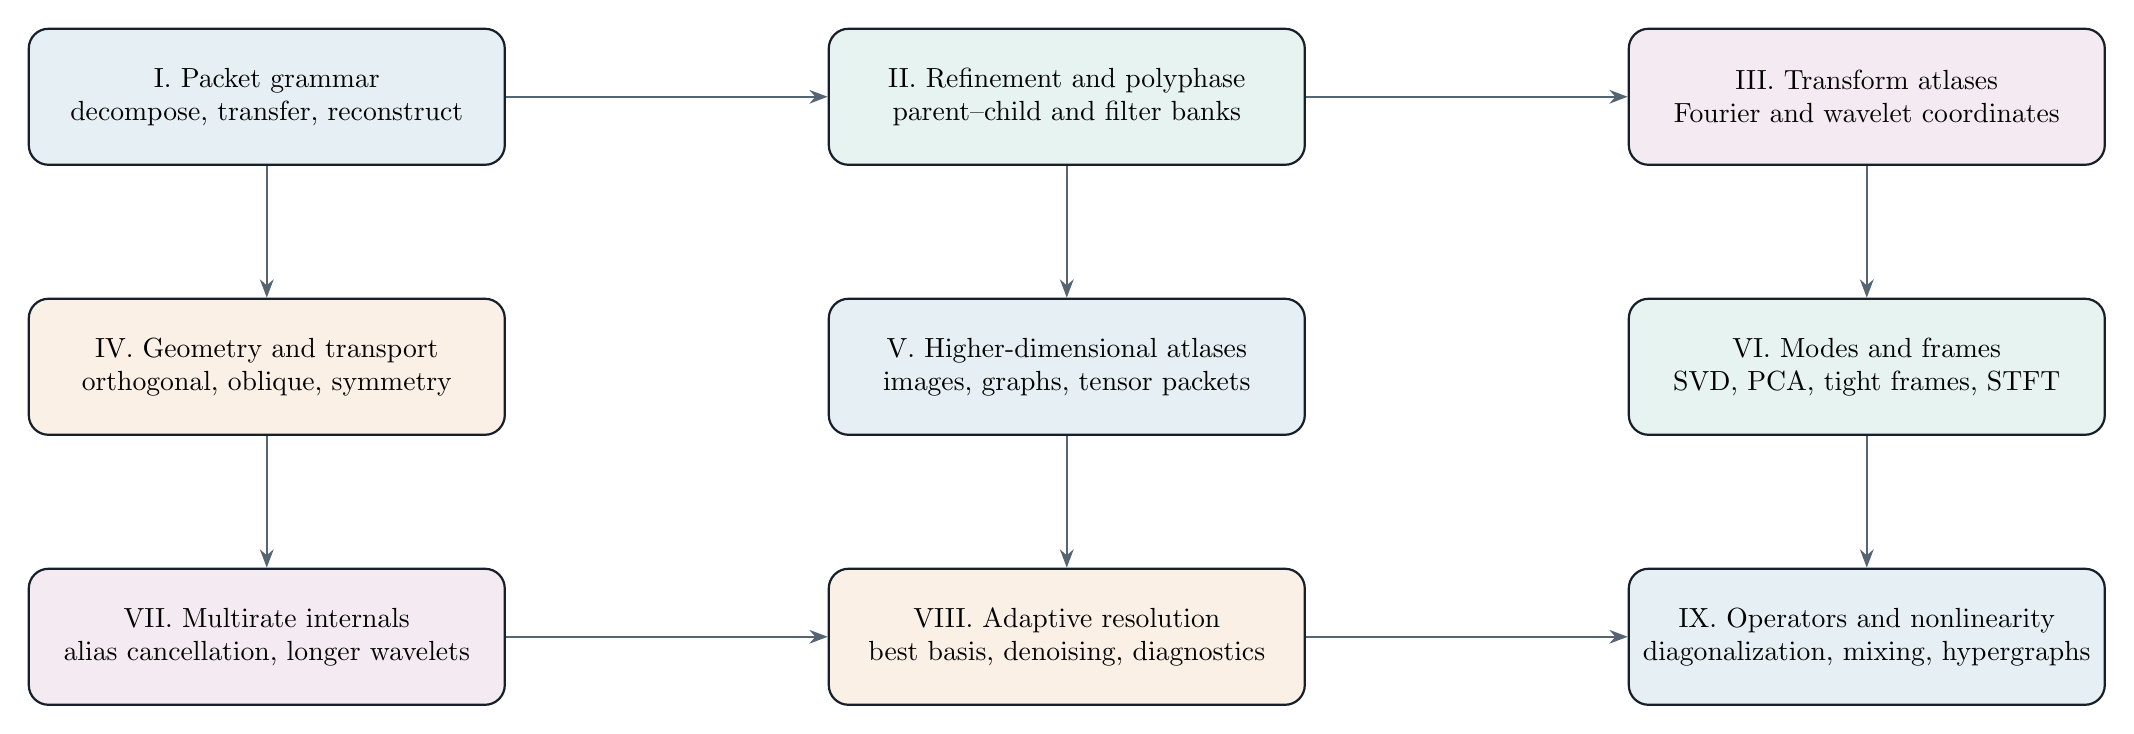
\begin{tikzpicture}[x=1in,y=1in,>=Stealth,
 box/.style={rounded corners=2.5mm,draw=Ink,thick,minimum width=2.38in,minimum height=.68in,align=center,font=\normalsize},
 arr/.style={->,thick,draw=Muted}]
\node[box,fill=PaleBlue] at (0,2.15) (core) {I. Packet grammar\\decompose, transfer, reconstruct};
\node[box,fill=PaleTeal] at (4.0,2.15) (ref) {II. Refinement and polyphase\\parent--child and filter banks};
\node[box,fill=PaleMagenta] at (8.0,2.15) (trans) {III. Transform atlases\\Fourier and wavelet coordinates};
\node[box,fill=PaleOrange] at (0,0.80) (geom) {IV. Geometry and transport\\orthogonal, oblique, symmetry};
\node[box,fill=PaleBlue] at (4.0,0.80) (high) {V. Higher-dimensional atlases\\images, graphs, tensor packets};
\node[box,fill=PaleTeal] at (8.0,0.80) (modes) {VI. Modes and frames\\SVD, PCA, tight frames, STFT};
\node[box,fill=PaleMagenta] at (0,-0.55) (multi) {VII. Multirate internals\\alias cancellation, longer wavelets};
\node[box,fill=PaleOrange] at (4.0,-0.55) (adapt) {VIII. Adaptive resolution\\best basis, denoising, diagnostics};
\node[box,fill=PaleBlue] at (8.0,-0.55) (nonlin) {IX. Operators and nonlinearity\\diagonalization, mixing, hypergraphs};
\draw[arr] (core)--(ref); \draw[arr] (ref)--(trans);
\draw[arr] (core)--(geom); \draw[arr] (ref)--(high); \draw[arr] (trans)--(modes);
\draw[arr] (geom)--(multi); \draw[arr] (high)--(adapt); \draw[arr] (modes)--(nonlin);
\draw[arr] (multi)--(adapt); \draw[arr] (adapt)--(nonlin);
\end{tikzpicture}
\end{center}
\vspace{0.10in}
\TwoBox{PaleTeal}{\ExactBadge\quad A complete declared coordinate family is synthesized without omission. Numerical residuals certify each finite example.}{PaleOrange}{\ApproxBadge\quad Thresholding, pruning, denoising, sparse retention, or packet dropping is shown only after complete analysis.}
\vfill
\Callout[PaleMagenta]{The first three parts establish the common grammar. The expanded parts then answer a practical question: what else becomes visible once decomposition, refinement, transfer, and reconstruction are treated as one reusable coordinate mechanism?}


% 2
\clearpage
\PageTitle[ORIENTATION]{What this guide is meant to show}
\begin{center}
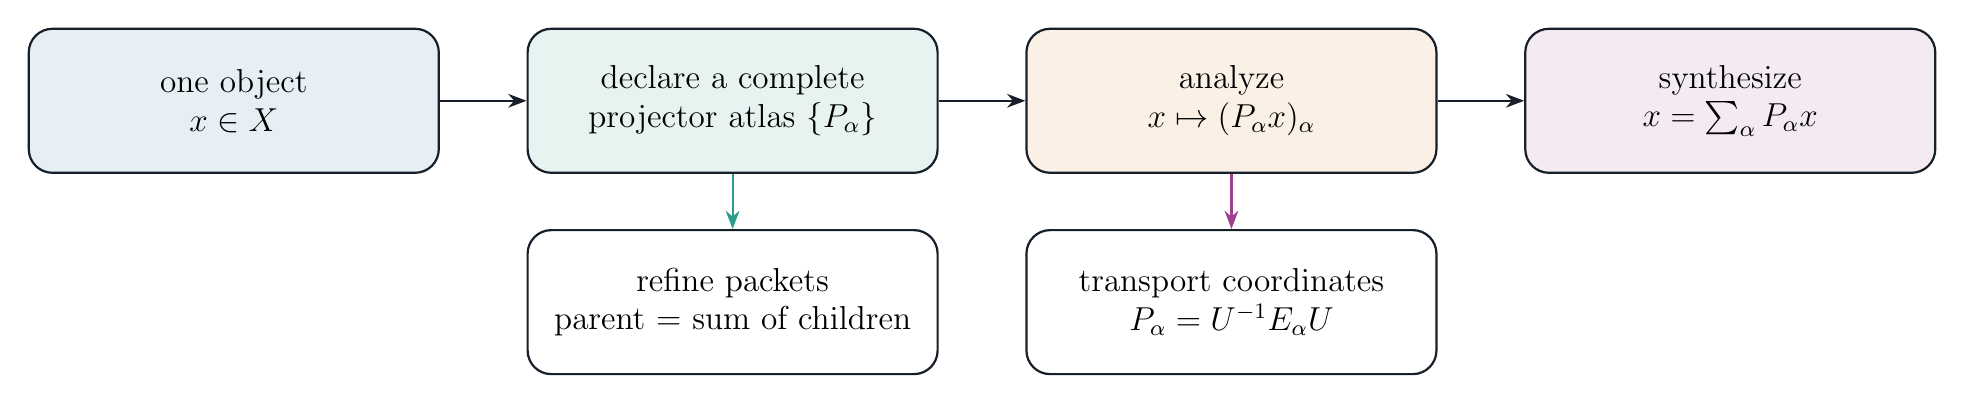
\begin{tikzpicture}[node distance=7mm and 11mm,>=Stealth,
  box/.style={rounded corners=3mm,draw=Ink,thick,minimum width=2.05in,minimum height=.72in,align=center,font=\large},
  arr/.style={->,thick,draw=Ink}]
\node[box,fill=PaleBlue] (x) {one object\\$x\in X$};
\node[box,fill=PaleTeal,right=of x] (p) {declare a complete\\projector atlas $\{P_\alpha\}$};
\node[box,fill=PaleOrange,right=of p] (a) {analyze\\$x\mapsto(P_\alpha x)_\alpha$};
\node[box,fill=PaleMagenta,right=of a] (s) {synthesize\\$x=\sum_\alpha P_\alpha x$};
\draw[arr] (x)--(p); \draw[arr] (p)--(a); \draw[arr] (a)--(s);
\node[box,fill=white,below=of p] (r) {refine packets\\parent $=$ sum of children};
\node[box,fill=white,below=of a] (t) {transport coordinates\\$P_\alpha=U^{-1}E_\alpha U$};
\draw[arr,draw=Teal] (p)--(r); \draw[arr,draw=Magenta] (a)--(t);
\end{tikzpicture}
\end{center}
\vspace{0.12in}
\TwoBox{PaleTeal}{\ExactBadge\quad Complete packets, complete Fourier bins, complete wavelet coordinates, all polyphase channels, and a perfect-reconstruction synthesis bank reproduce the object exactly.}{PaleOrange}{\ApproxBadge\quad Truncation, thresholding, denoising, and sparse retention begin only after a complete coordinate representation has been formed.}
\vfill
\Callout{The visual sequence proceeds from the universal packet identities to concrete residue channels, operator transfer blocks, refinement trees, polyphase filter banks, Fourier projectors, wavelet packet projectors, and composed atlases.}

% 3
\clearpage
\PageTitle[CLAIM CONTROL]{What is structural, what is classical, and what is numerical}
\begin{tabularx}{\linewidth}{>{\bfseries}p{1.75in} X X}
\toprule
Layer & Exact statement used in this guide & Status \tabularnewline
\midrule
Projector calculus & $P_\alpha P_\beta=\delta_{\alpha\beta}P_\alpha$, $\sum_\alpha P_\alpha=I$, hence $x=\sum_\alpha P_\alpha x$ and $T=\sum_{\alpha,\beta}P_\beta TP_\alpha$. & Algebraic identity once a complete packet system is declared.\\
Transform atlas & For invertible $U$ and coordinate selectors $E_\alpha$, set $P_\alpha=U^{-1}E_\alpha U$. Packet and transfer laws follow by conjugation. & Classical linear algebra used as the framework's coordinate-transport rule.\\
Fourier and wavelets & $U=F$ gives Fourier packets; $U=W$ gives wavelet or wavelet-packet coordinates. If $U$ is unitary, energy is preserved. & Classical transforms represented inside the common projector language.\\
Polyphase refinement & Address classes are exact packets; interleaving inverts extraction. Filter-bank perfect reconstruction is $R(z)E(z)=z^{-d}I$. & Classical multirate identities written as packet analysis and synthesis.\\
Approximation examples & Some coordinates are discarded to compare Fourier truncation, wavelet sparsification, and edge-aware packets. & Numerical demonstrations, not exact reconstruction claims.\\
\bottomrule
\end{tabularx}
\vfill
\Callout[PaleMagenta]{The unifying content is not that Fourier analysis or wavelets are newly invented. It is that they become instances of the same analysis--synthesis, refinement, and transfer-block grammar.}

% 4
\VisualPage[4.95in]{THE COMMON GRAMMAR}{One operator language, many realizations}{01_framework_pipeline.pdf}{Every realization supplies projectors, analysis, synthesis, and transfer blocks. Changing the atlas changes what is easy to see, but a complete atlas preserves the object and the operator.}

% 5
\VisualPage[4.92in]{PACKET AXIOMS}{A decomposition begins with a complete packet system}{02_packet_identities.pdf}{The algebraic core is pairwise annihilation and completeness. Orthogonality adds geometry and energy identities, but exact synthesis already follows from $\sum_iP_i=I$.}

% 6
\VisualPage[4.92in]{ANALYSIS AND SYNTHESIS}{The coordinate tuple is equivalent to the object}{03_analysis_synthesis.pdf}{Analysis stores every packet component; synthesis adds them. On the complete packet range, both compositions are identities.}

% 7
\VisualPage[4.92in]{A CONCRETE DECOMPOSITION}{Residue packets separate addresses without losing samples}{04_signal_packet_decomposition.pdf}{For $P_{N,r}$, packet $r$ keeps samples whose addresses satisfy $n\equiv r\pmod N$. The support patterns are disjoint and their union is the whole signal.}

% 8
\VisualPage[4.92in]{EXACT RECONSTRUCTION}{Synthesis interleaves the complete family exactly}{05_exact_reconstruction.pdf}{The plotted reconstruction overlays the original signal. The residual is zero to floating-point precision because no phase packet was omitted.}

% 9
\VisualPage[4.92in]{OPERATOR DECOMPOSITION}{Every operator splits into input-to-output transfer blocks}{06_transfer_blocks.pdf}{The block $T_{\beta\alpha}=P_\beta T P_\alpha$ records the part of the operator that carries input packet $\alpha$ into output packet $\beta$. Summing all blocks reconstructs $T$.}

% 10
\VisualPage[4.90in]{TRANSFER PATHS}{Operator products become sums over packet paths}{07_transfer_paths.pdf}{Inserting $I=\sum_\gamma P_\gamma$ between operators turns composition into a path sum. Iterated products are resolved by all admissible intermediate packet addresses.}

% 11
\clearpage
\PageTitle[REFINEMENT]{A packet address can be made finer without changing the object}
\begin{center}
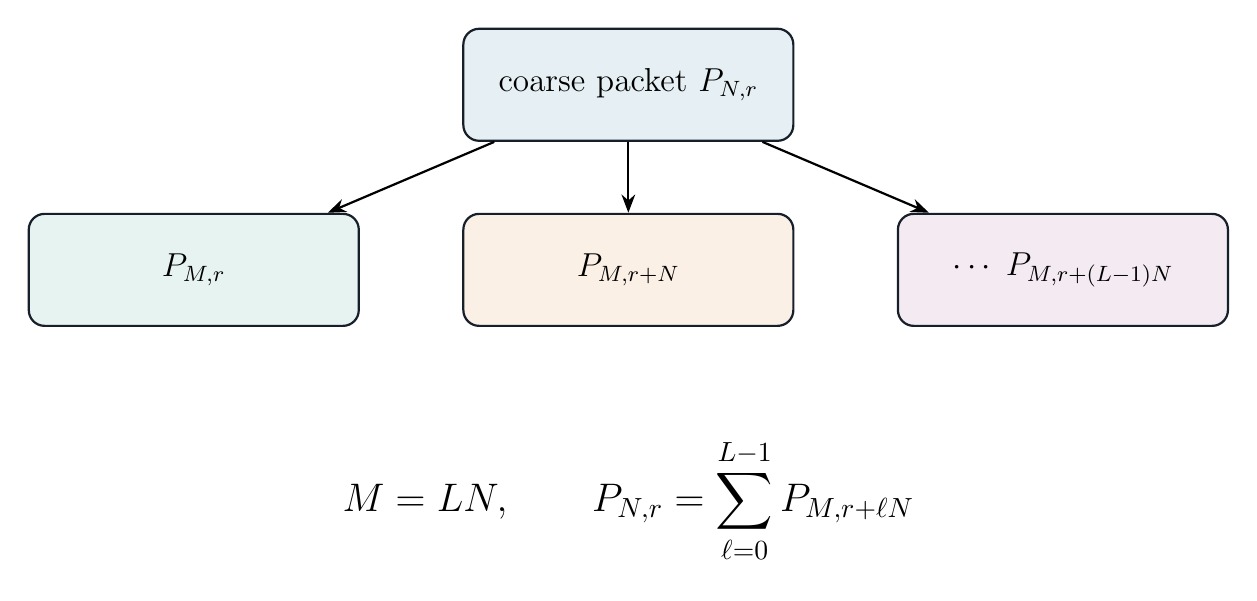
\begin{tikzpicture}[>=Stealth,node distance=9mm and 13mm,
 p/.style={rounded corners=2mm,draw=Ink,thick,minimum width=1.65in,minimum height=.56in,align=center,font=\large}]
\node[p,fill=PaleBlue] (c) {coarse packet $P_{N,r}$};
\node[p,fill=PaleTeal,below left=of c] (f0) {$P_{M,r}$};
\node[p,fill=PaleOrange,below=of c] (f1) {$P_{M,r+N}$};
\node[p,fill=PaleMagenta,below right=of c] (f2) {$\cdots\;P_{M,r+(L-1)N}$};
\draw[->,thick] (c)--(f0); \draw[->,thick] (c)--(f1); \draw[->,thick] (c)--(f2);
\node[below=13mm of f1,font=\Large] {$M=LN,\qquad P_{N,r}=\displaystyle\sum_{\ell=0}^{L-1}P_{M,r+\ell N}$};
\end{tikzpicture}
\end{center}
\vspace{0.20in}
\TwoBox{PaleTeal}{\bfseries Analysis refinement.\par The fine coordinate tuple is obtained from the coarse tuple by resolving each parent into its children.}{PaleOrange}{\bfseries Synthesis coarsening.\par The parent coordinate is recovered by summing or synthesizing all of its children.}
\vfill
\Callout{Refinement is exact when every child is retained. It becomes approximation only when children are merged, averaged, thresholded, or discarded.}

% 12
\VisualPage[4.92in]{REFINEMENT TREE}{Polyphase refinement is a parent--child decomposition}{08_refinement_tree.pdf}{A residue packet modulo $N$ splits into residue packets modulo $M=LN$. The tree shows address refinement, not a change to the underlying signal.}

% 13
\VisualPage[4.92in]{REFINEMENT MAPS}{Coarse and fine coordinates are linked by inverse maps}{09_refinement_maps.pdf}{The maps $J=\mathcal A_{\mathrm f}\mathcal S_{\mathrm c}$ and $C=\mathcal A_{\mathrm c}\mathcal S_{\mathrm f}$ translate between complete coordinate atlases. Their compositions are identities on the represented packet ranges.}

% 14
\VisualPage[4.92in]{BLOCK REFINEMENT}{A coarse transfer block is the sum of its fine child blocks}{10_operator_block_refinement.pdf}{Refining both input and output packets produces a matrix of child-to-child blocks. Summing that matrix recovers the coarse block exactly.}

% 15
\VisualPage[4.92in]{POLYPHASE ANALYSIS}{Extraction separates address classes and decimates each channel}{11_polyphase_analysis.pdf}{The polyphase analysis map is $\mathcal A_Nx=(x_0,\ldots,x_{N-1})$ with $x_r[q]=x[Nq+r]$. Each original sample appears in exactly one channel.}

% 16
\VisualPage[4.92in]{POLYPHASE SYNTHESIS}{Interleaving is the inverse of channel extraction}{12_polyphase_synthesis.pdf}{$\mathcal S_N$ returns each channel value to its original address. Thus $\mathcal S_N\mathcal A_N=I$ for the complete channel family.}

% 17
\VisualPage[4.92in]{POLYPHASE OPERATOR MATRIX}{A convolution becomes a matrix of channel-to-channel filters}{13_fir_polyphase_matrix.pdf}{Conjugating a finite impulse-response operator by polyphase analysis and synthesis yields $\mathcal A_NH\mathcal S_N=[H^{(N)}_{ks}(z)]_{k,s}$. Each cell is a transfer block between phase packets.}

% 18
\VisualPage[4.92in]{PERFECT RECONSTRUCTION}{Analysis and synthesis banks cancel as an operator identity}{14_perfect_reconstruction_bank.pdf}{A filter bank is perfectly reconstructing when $\mathbf R(z)\mathbf E(z)=z^{-d}I_N$. The only permitted change is the declared delay $d$; every channel vector is otherwise recovered.}

% 19
\clearpage
\PageTitle[POLYPHASE FORMULAS]{The multirate identities in one place}
\begin{minipage}[t]{0.48\linewidth}
\colorbox{PaleTeal}{\parbox{0.94\linewidth}{
\vspace{7pt}
\textbf{Address projectors}\par
\[
(P_{N,r}x)[n]=\mathbf 1_{n\equiv r\ (\mathrm{mod}\ N)}x[n],\qquad
\sum_{r=0}^{N-1}P_{N,r}=I.
\]
\textbf{Analysis and synthesis}\par
\[
x_r[q]=x[Nq+r],\qquad
(\mathcal S_N(x_0,\ldots,x_{N-1}))[Nq+r]=x_r[q].
\]
\[
\mathcal S_N\mathcal A_N=I.
\]
\vspace{6pt}}}
\end{minipage}\hfill
\begin{minipage}[t]{0.48\linewidth}
\colorbox{PaleOrange}{\parbox{0.94\linewidth}{
\vspace{7pt}
\textbf{Refinement}\par
\[
M=LN\quad\Longrightarrow\quad
P_{N,r}=\sum_{\ell=0}^{L-1}P_{M,r+\ell N}.
\]
\textbf{Operator and filter-bank forms}\par
\[
\mathcal A_NT\mathcal S_N=[P_{N,k}TP_{N,s}]_{k,s},
\qquad
\mathbf R(z)\mathbf E(z)=z^{-d}I_N.
\]
\vspace{6pt}}}
\end{minipage}
\vspace{0.26in}
\Callout[PaleMagenta]{Polyphase analysis is therefore not external to projector calculus: it is the coordinate analysis associated with residue-class projectors. Its filter matrices are the corresponding transfer-block matrices.}

% 20
\clearpage
\PageTitle[WAVELET REALIZATIONS]{Wavelets enter through an invertible or unitary transform atlas}
\begin{center}
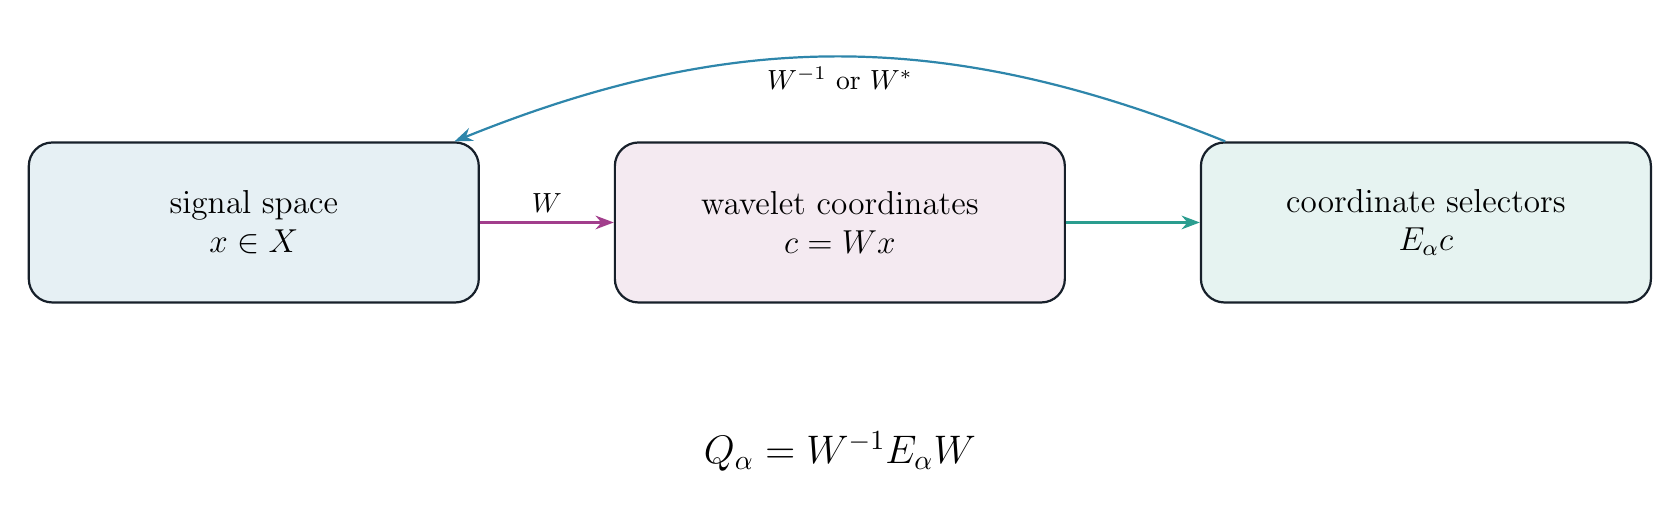
\begin{tikzpicture}[>=Stealth,node distance=11mm and 17mm,
 box/.style={rounded corners=3mm,draw=Ink,thick,minimum width=2.25in,minimum height=.80in,align=center,font=\large}]
\node[box,fill=PaleBlue] (x) {signal space\\$x\in X$};
\node[box,fill=PaleMagenta,right=of x] (w) {wavelet coordinates\\$c=Wx$};
\node[box,fill=PaleTeal,right=of w] (e) {coordinate selectors\\$E_\alpha c$};
\draw[->,thick,draw=Magenta] (x)--node[above] {$W$} (w);
\draw[->,thick,draw=Teal] (w)--(e);
\draw[->,thick,draw=Blue,bend right=22] (e) to node[below] {$W^{-1}$ or $W^*$} (x);
\node[below=15mm of w,font=\Large] {$Q_\alpha=W^{-1}E_\alpha W$};
\end{tikzpicture}
\end{center}
\vspace{0.18in}
\TwoBox{PaleTeal}{\ExactBadge\quad Keeping every coefficient selector gives $\sum_\alpha Q_\alpha=I$ and exact inverse-wavelet reconstruction.}{PaleOrange}{\ApproxBadge\quad Thresholding or keeping only selected packets gives a sparse or denoised approximation.}
\vfill
\Callout{For an orthogonal wavelet transform, $W^{-1}=W^*$ and $\|x\|^2=\sum_\alpha\|Q_\alpha x\|^2$.}

% 21
\VisualPage[4.92in]{HAAR ANALYSIS}{The Haar bank is a two-packet unitary realization}{15_haar_decomposition.pdf}{The low and detail channels are linear coordinate packets. Both are needed for exact reconstruction; neither is intrinsically “signal” or “noise.”}

% 22
\VisualPage[4.92in]{HAAR SYNTHESIS}{The two packets reproduce every sample and partition energy}{16_haar_reconstruction_energy.pdf}{With the orthonormal Haar normalization, synthesis is the transpose of analysis and Parseval's identity holds exactly up to floating-point roundoff.}

% 23
\VisualPage[4.92in]{LIFTING}{An exact wavelet transform can factor into reversible local steps}{17_lifting_scheme.pdf}{Split, predict, update, and scale form elementary invertible operators. Reversing the order and signs reconstructs the original samples.}

% 24
\VisualPage[4.92in]{WAVELET PACKETS}{Both children can be refined recursively}{18_wavelet_packet_tree.pdf}{Wavelet-packet addresses combine scale and branch history. The leaves form a complete coordinate atlas when every branch at the chosen depth is retained.}

% 25
\VisualPage[4.92in]{WAVELET ATOMS}{Packet coordinates are localized oscillatory basis directions}{19_wavelet_packet_atoms.pdf}{Rows of the orthogonal transform are coordinate atoms. Pulling individual coefficient selectors back through the transform creates exact projectors in signal space.}

% 26
\VisualPage[4.92in]{WAVELET REFINEMENT}{A parent packet equals the synthesis of its two children}{27_wavelet_refinement_identity.pdf}{Refining a parent does not create or destroy information. The parent contribution is the exact sum of the synthesized child contributions.}

% 27
\clearpage
\PageTitle[TRANSFORM ATLASES]{A single conjugation rule contains Fourier and wavelet coordinates}
\begin{center}
\colorbox{PaleBlue}{\parbox{0.88\linewidth}{
\vspace{8pt}
\begin{center}
\Large\bfseries Transform-atlas proposition
\end{center}
Let $U:X\to Y$ be invertible, and let $\{E_\alpha\}$ be coordinate selectors on $Y$ satisfying
\[
E_\alpha E_\beta=\delta_{\alpha\beta}E_\alpha,
\qquad \sum_\alpha E_\alpha=I_Y.
\]
Define
\[
P_\alpha=U^{-1}E_\alpha U.
\]
Then $\{P_\alpha\}$ is a complete packet system on $X$, and for every object $x$ and operator $T$,
\[
x=\sum_\alpha P_\alpha x,
\qquad
T=\sum_{\alpha,\beta}P_\beta TP_\alpha.
\]
If $U$ is unitary, then $\|x\|^2=\sum_\alpha\|P_\alpha x\|^2$.
\vspace{8pt}}}
\end{center}
\vspace{0.15in}
\begin{center}
\begin{tabular}{lll}
\toprule
Choice of $U$ & Coordinate selectors & Pulled-back packets \\
\midrule
$F$ (unitary DFT) & bins or disjoint frequency bands & $F^*E_BF$ \\
$W$ (orthogonal wavelet transform) & scale--location or packet coefficients & $W^*E_\alpha W$ \\
$\mathcal A_N$ (polyphase isomorphism) & channel coordinates & $P_{N,r}$ and channel blocks \\
any invertible atlas & ordinary coordinate axes & $U^{-1}E_\alpha U$ \\
\bottomrule
\end{tabular}
\end{center}

% 28
\VisualPage[4.92in]{THE GENERIC CONSTRUCTION}{Coordinate selectors pull back to object-space projectors}{20_transform_atlas_principle.pdf}{Fourier and wavelet space are therefore not outside the framework. They are coordinate spaces whose ordinary selectors become object-space packets by conjugation.}

% 29
\VisualPage[4.92in]{FOURIER SPACE}{Frequency bands form a complete projector atlas}{21_fourier_projectors.pdf}{With the unitary DFT $F$, a disjoint complete cover of frequency bins gives $Q_B=F^*E_BF$ and $x=\sum_BQ_Bx$.}

% 30
\VisualPage[4.92in]{FOURIER CHARACTER PROJECTORS}{Cyclic symmetry also constructs the frequency packets directly}{22_fourier_character_projector.pdf}{For the cyclic shift $U$, the character average $P_{N,j}=N^{-1}\sum_{m=0}^{N-1}\omega^{-jm}U^m$ isolates one frequency character. This is the finite spectral projector formula.}

% 31
\VisualPage[4.92in]{WAVELET SPACE}{Coefficient selectors pull back to scale--location projectors}{23_wavelet_projectors.pdf}{For an orthogonal wavelet-packet matrix $W$, $Q_\alpha=W^*E_\alpha W$ is idempotent, distinct packets annihilate, and the complete sum is the identity.}

% 32
\VisualPage[4.92in]{TWO EXACT COORDINATE SYSTEMS}{Fourier and wavelets represent the same object differently}{24_fourier_wavelet_coordinates.pdf}{Fourier coordinates emphasize global oscillation. Wavelet coordinates emphasize scale and location. With all coefficients present, both synthesize the identical signal.}

% 33
\VisualPage[4.92in]{THE SAME OPERATOR IN THREE ATLASES}{Coordinate transport changes sparsity patterns, not the operator}{25_operator_in_three_atlases.pdf}{$T$, $FTF^*$, and $WTW^*$ are coordinate representations of one operator. A useful atlas is often the one in which the relevant transfer blocks become sparse, localized, or structured.}

% 34
\VisualPage[4.92in]{COMPOSED COORDINATES}{Polyphase and Fourier addresses can coexist}{26_phase_frequency_lattice.pdf}{First separate phases, then Fourier-analyze each decimated channel. The resulting address $(r,k)$ records both residue phase and within-channel frequency, and the inverse composition is exact.}

% 35
\clearpage
\PageTitle[EXACTNESS BOUNDARY]{Complete coordinates reconstruct; selected coordinates approximate}
\begin{center}
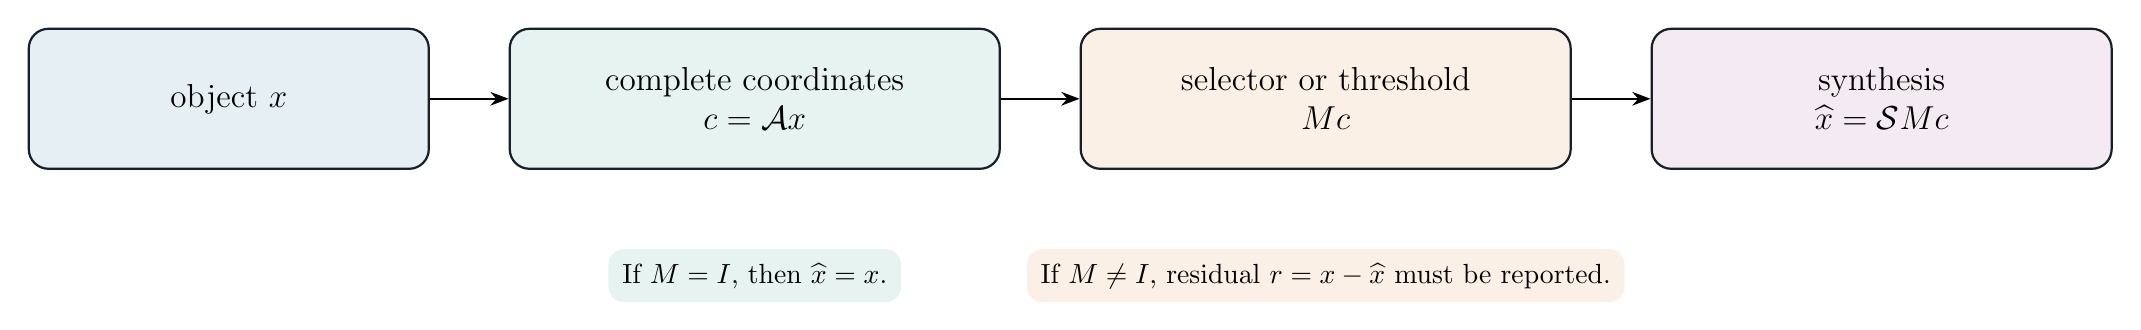
\begin{tikzpicture}[>=Stealth,node distance=8mm and 10mm,
 b/.style={rounded corners=2.5mm,draw=Ink,thick,minimum height=.70in,align=center,font=\large}]
\node[b,fill=PaleBlue,minimum width=2.0in] (x) {object $x$};
\node[b,fill=PaleTeal,right=of x,minimum width=2.45in] (c) {complete coordinates\\$c=\mathcal A x$};
\node[b,fill=PaleOrange,right=of c,minimum width=2.45in] (sel) {selector or threshold\\$Mc$};
\node[b,fill=PaleMagenta,right=of sel,minimum width=2.30in] (xh) {synthesis\\$\widehat x=\mathcal S Mc$};
\draw[->,thick] (x)--(c); \draw[->,thick] (c)--(sel); \draw[->,thick] (sel)--(xh);
\node[below=10mm of c,fill=PaleTeal,rounded corners=2mm,inner sep=5pt] {If $M=I$, then $\widehat x=x$.};
\node[below=10mm of sel,fill=PaleOrange,rounded corners=2mm,inner sep=5pt] {If $M\neq I$, residual $r=x-\widehat x$ must be reported.};
\end{tikzpicture}
\end{center}
\vspace{0.15in}
\TwoBox{PaleTeal}{\bfseries Exact coordinate change\par all packets, all Fourier bins, all wavelet coefficients, all polyphase channels, or an exactly invertible lifting/filter-bank chain.}{PaleOrange}{\bfseries Deliberate compression\par Fourier truncation, coefficient thresholding, best-basis pruning, packet dropping, model-based edge retention, or coarse-only reconstruction.}
\vfill
\Callout{The framework does not make a lossy selection exact. It makes the location of loss explicit: loss enters through $M$, not through the complete analysis or synthesis maps.}

% 36
\VisualPage[4.92in]{EXACT VERSUS APPROXIMATE}{The guide marks where information is discarded}{28_exact_vs_approximate.pdf}{The certificate matrix distinguishes complete coordinate identities from examples that intentionally suppress coordinates.}

% 37
\VisualPage[4.92in]{EDGE EXAMPLE}{Different atlases concentrate an edge differently}{29_edge_reconstruction_comparison.pdf}{Global Fourier truncation spreads a discontinuity across global modes. Wavelet and edge-aware packets can concentrate the same structure more locally. The displayed incomplete reconstructions are approximations.}

% 38
\VisualPage[4.92in]{SPARSE RETENTION}{Fourier and wavelet errors depend on how many coefficients are kept}{30_sparse_fourier_wavelet.pdf}{This finite example compares equal coefficient budgets. It illustrates coordinate concentration, not a universal dominance theorem.}

% 39
\VisualPage[4.92in]{TWO-DIMENSIONAL EXTENSION}{The same packet logic applies to images and fields}{31_two_dimensional_edge_packet.pdf}{A 2D object can be resolved by spatial, Fourier, wavelet, geometric, or learned-but-invertible atlases. The exact law remains $x=\sum_\alpha P_\alpha x$ when the packet family is complete.}

% 40
\VisualPage[4.92in]{THE UNIFIED VIEW}{Several exact atlases may resolve one object}{32_unified_atlas.pdf}{Polyphase, Fourier, wavelet, and other invertible coordinates coexist as different projector atlases. Each has its own analysis and synthesis maps but obeys the same packet and transfer-block laws.}

% 41
\VisualPage[4.92in]{THE VISUAL GRAMMAR}{Decomposition, transfer, refinement, and transport form one wheel}{33_summary_wheel.pdf}{The wheel summarizes the operations that recur throughout the guide. No one atlas is privileged in advance; the problem determines which packet geometry is most informative.}

% 42
\VisualPage[4.92in]{NUMERICAL CERTIFICATES}{Every exact finite example was checked by a residual}{34_verification_dashboard.pdf}{Zero-valued identities are exact in the implemented finite model; residuals near $10^{-14}$ are floating-point roundoff. Approximation errors are reported separately and are not labeled as exact.}


% Expanded Part IV
\clearpage
\PageTitle[EXPANDED PART IV]{Geometry, transport, and compatibility}
\begin{minipage}[t]{0.47\linewidth}
\colorbox{PaleBlue}{\parbox{0.94\linewidth}{
\vspace{7pt}
\textbf{Orthogonal packet geometry}
\[
P_i^2=P_i=P_i^*,\qquad P_iP_j=0,
\qquad \sum_iP_i=I.
\]
Then
\[
x=\sum_iP_ix,
\qquad
\|x\|^2=\sum_i\|P_ix\|^2.
\]
\vspace{5pt}}}
\end{minipage}\hfill
\begin{minipage}[t]{0.47\linewidth}
\colorbox{PaleOrange}{\parbox{0.94\linewidth}{
\vspace{7pt}
\textbf{Oblique but exact geometry}
\[
P_i^2=P_i,\qquad P_iP_j=0,
\qquad \sum_iP_i=I,
\]
while generally $P_i\ne P_i^*$. Exact synthesis survives, but Pythagorean energy additivity need not.
\vspace{5pt}}}
\end{minipage}
\vspace{0.18in}
\begin{center}
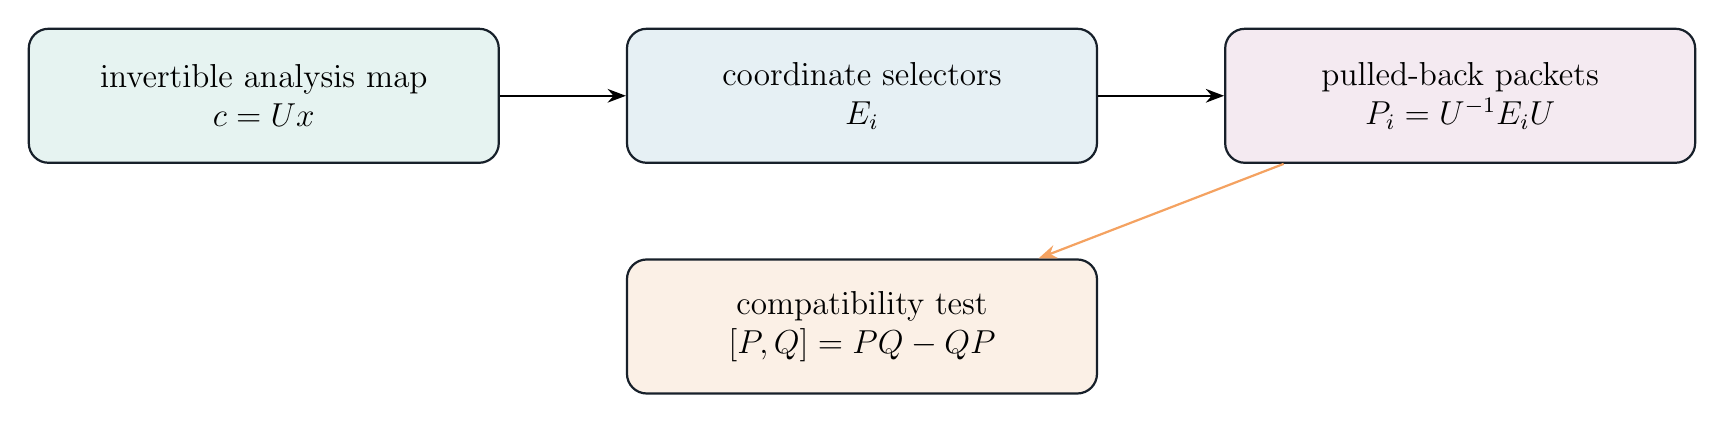
\begin{tikzpicture}[>=Stealth,node distance=12mm and 16mm,
 box/.style={rounded corners=2.5mm,draw=Ink,thick,minimum width=2.35in,minimum height=.67in,align=center,font=\large}]
\node[box,fill=PaleTeal] (u) {invertible analysis map\\$c=Ux$};
\node[box,fill=PaleBlue,right=of u] (e) {coordinate selectors\\$E_i$};
\node[box,fill=PaleMagenta,right=of e] (p) {pulled-back packets\\$P_i=U^{-1}E_iU$};
\draw[->,thick] (u)--(e); \draw[->,thick] (e)--(p);
\node[box,fill=PaleOrange,below=of e] (c) {compatibility test\\$[P,Q]=PQ-QP$};
\draw[->,thick,draw=Orange] (p)--(c);
\end{tikzpicture}
\end{center}
\vfill
\Callout{A complete atlas answers whether reconstruction is possible. Orthogonality answers whether energy is additive. Conditioning answers whether the reconstruction is numerically stable. Commutation answers whether two packet systems admit a straightforward joint refinement.}

\VisualPage[4.82in]{PROJECTOR GEOMETRY}{Rank-one packets make the decomposition visible as vector addition}{35_rank_one_projector_geometry.pdf}{The simplest geometric picture already contains the full law: complementary packet components add to the original vector, while annihilation and completeness appear directly in the projector matrices.}

\VisualPage[4.82in]{BEYOND ORTHOGONALITY}{Oblique projectors can reconstruct exactly without a Pythagorean energy split}{36_orthogonal_vs_oblique.pdf}{Both panels satisfy $x=P_1x+P_2x$. Only the orthogonal panel satisfies the usual sum-of-squared-component-norms identity. This separates algebraic exactness from metric geometry.}

\VisualPage[4.82in]{STABILITY}{Invertibility guarantees a formula; conditioning governs sensitivity}{37_atlas_conditioning.pdf}{The unperturbed coordinate solve remains exact. A small coordinate perturbation is amplified as the atlas becomes increasingly skew, making the condition number part of a responsible reconstruction certificate.}

\VisualPage[4.82in]{ATLAS-TO-ATLAS TRANSPORT}{Fourier coordinates can be converted directly into wavelet coordinates}{38_fourier_wavelet_transition.pdf}{For unitary $F$ and $W$, the transition map is $WF^*$. It is itself unitary and transports a complete Fourier coordinate tuple into a complete wavelet-packet tuple without returning first to an informal representation.}

\VisualPage[4.82in]{COMPATIBILITY}{Commuting projectors refine cleanly; noncommuting projectors remember order}{39_commuting_vs_noncommuting.pdf}{Residue and Fourier selectors are each legitimate packets, but they need not commute. When $PQ\ne QP$, sequential selection depends on order and a naive intersection picture is insufficient.}

\VisualPage[4.82in]{SYMMETRY PACKETS}{Reflection splits an object into even and odd components}{40_reflection_symmetry_packets.pdf}{The involution $R^2=I$ produces $P_{+}=(I+R)/2$ and $P_{-}=(I-R)/2$. Their sum is the identity, their product is zero, and synthesis recovers the asymmetric original exactly.}

% Expanded Part V
\clearpage
\PageTitle[EXPANDED PART V]{Higher-dimensional, graph, and data-adapted atlases}
\begin{center}
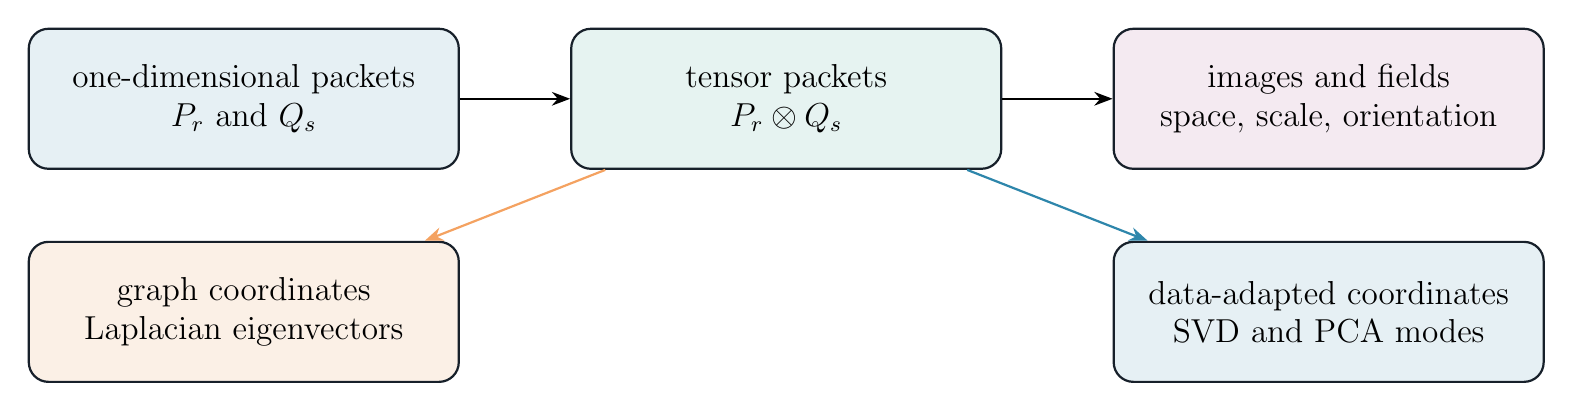
\begin{tikzpicture}[>=Stealth,node distance=9mm and 14mm,
 box/.style={rounded corners=2.5mm,draw=Ink,thick,minimum width=2.15in,minimum height=.70in,align=center,font=\large}]
\node[box,fill=PaleBlue] (one) {one-dimensional packets\\$P_r$ and $Q_s$};
\node[box,fill=PaleTeal,right=of one] (tensor) {tensor packets\\$P_r\otimes Q_s$};
\node[box,fill=PaleMagenta,right=of tensor] (image) {images and fields\\space, scale, orientation};
\draw[->,thick] (one)--(tensor); \draw[->,thick] (tensor)--(image);
\node[box,fill=PaleOrange,below left=of tensor] (graph) {graph coordinates\\Laplacian eigenvectors};
\node[box,fill=PaleBlue,below right=of tensor] (data) {data-adapted coordinates\\SVD and PCA modes};
\draw[->,thick,draw=Orange] (tensor)--(graph); \draw[->,thick,draw=Blue] (tensor)--(data);
\end{tikzpicture}
\end{center}
\vspace{0.14in}
\TwoBox{PaleTeal}{\textbf{Product construction.}\par Complete one-dimensional packet systems produce a complete product family: $\sum_{r,s}P_r\otimes Q_s=I\otimes I$.}{PaleMagenta}{\textbf{Spectral construction.}\par Any real symmetric operator, covariance matrix, or graph Laplacian supplies orthogonal eigencoordinates and spectral selectors.}
\vfill
\Callout{The coordinate labels need not be points on a line. They may be pixel addresses, scale--orientation cells, graph eigenmodes, singular modes of a matrix, or principal directions learned from covariance.}

\VisualPage[4.82in]{TENSOR PRODUCTS}{One-dimensional address packets become a complete two-dimensional grid}{41_tensor_product_packets.pdf}{The packet indexed by $(r,s)$ keeps exactly the coordinates whose row and column addresses lie in the selected residue classes. Summing every tensor packet restores the full array.}

\VisualPage[4.82in]{TWO-DIMENSIONAL WAVELETS}{A separable Haar atlas resolves average, horizontal, vertical, and diagonal structure}{42_two_dimensional_haar_subbands.pdf}{The four subbands are complete orthogonal coordinates for one level of a 2D Haar transform. Their energy bars show how the chosen image distributes energy across scale and orientation.}

\VisualPage[4.82in]{TWO-DIMENSIONAL SYNTHESIS}{Each wavelet subband pulls back to an object-space image packet}{43_two_dimensional_haar_reconstruction.pdf}{Synthesizing one subband at a time reveals its object-space contribution. Adding LL, LH, HL, and HH reproduces the original image to floating-point roundoff.}

\VisualPage[4.82in]{TWO-DIMENSIONAL FOURIER SPACE}{Radial and angular masks define exact spectral tiles}{44_two_dimensional_fourier_tiles.pdf}{The displayed low-frequency disk and complementary angular sectors are disjoint and complete. Their inverse transforms are Fourier packets whose sum is the original image.}

\VisualPage[4.82in]{GRAPH FOURIER SPACE}{A graph Laplacian supplies frequencies without a regular grid}{45_graph_fourier_modes.pdf}{The Laplacian eigenvectors are the graph analogue of Fourier modes. Low eigenvalues vary slowly across strongly connected nodes; higher modes oscillate more rapidly across graph edges.}

\VisualPage[4.82in]{GRAPH SPECTRAL PACKETS}{Disjoint eigenvalue bands reconstruct a signal on a network}{46_graph_spectral_packets.pdf}{Selecting groups of graph eigenvectors creates pulled-back graph-frequency projectors. The four displayed bands sum to the identity on the twelve-node graph.}

% Expanded Part VI
\clearpage
\PageTitle[EXPANDED PART VI]{Mode decompositions and redundant analysis--synthesis systems}
\begin{minipage}[t]{0.47\linewidth}
\colorbox{PaleBlue}{\parbox{0.94\linewidth}{
\vspace{7pt}
\textbf{Orthogonal data modes}
\[
M=\sum_j\sigma_j u_jv_j^*,
\qquad
x-\bar x=\sum_j\langle x-\bar x,v_j\rangle v_j.
\]
SVD and PCA are classical coordinate systems selected by a matrix or covariance operator.
\vspace{5pt}}}
\end{minipage}\hfill
\begin{minipage}[t]{0.47\linewidth}
\colorbox{PaleOrange}{\parbox{0.94\linewidth}{
\vspace{7pt}
\textbf{Redundant frames}
\[
c_i=\langle x,f_i\rangle,
\qquad
x=\sum_i c_i\widetilde f_i.
\]
A frame may use more coordinates than the dimension. Exact synthesis uses a compatible dual frame rather than pairwise-annihilating projectors.
\vspace{5pt}}}
\end{minipage}
\vspace{0.22in}
\begin{center}
\ClassicalBadge\qquad The next examples extend the common analysis--synthesis grammar, while explicitly marking which systems are not disjoint projector atlases.
\end{center}
\vfill
\Callout[PaleMagenta]{The framework is broad enough to compare projectors, orthogonal modes, and redundant frames, but it should not erase their differences. The reconstruction operator and the status of the coordinates must be declared in each case.}

\VisualPage[4.82in]{MATRIX MODES}{SVD resolves a matrix into rank-one singular packets}{47_svd_mode_atlas.pdf}{For the constructed rank-three matrix, the first three singular modes synthesize the object exactly. Truncating the sum would turn the same decomposition into a low-rank approximation.}

\VisualPage[4.82in]{STATISTICAL COORDINATES}{PCA chooses an orthogonal atlas from the covariance structure}{48_pca_coordinate_atlas.pdf}{Centered observations are rotated into principal coordinates, variance is partitioned by eigenvalue, and multiplying by the transpose of the eigenvector matrix returns the original observations.}

\VisualPage[4.82in]{REDUNDANT FRAMES}{Three analysis vectors can represent a two-dimensional object exactly}{49_redundant_tight_frame.pdf}{This tight frame has redundant coefficients and exact dual-frame synthesis. It belongs to the broader analysis--synthesis grammar, but its individual rank-one terms are not a pairwise-annihilating complete projector family.}

\VisualPage[4.82in]{LOCAL FOURIER COORDINATES}{Short-time Fourier analysis uses overlapping time--frequency packets}{50_short_time_fourier_frame.pdf}{Window overlap creates redundant coordinates. Compatible synthesis windows perform overlap--add reconstruction exactly, giving a localized Fourier realization beyond a single global basis.}

% Expanded Part VII
\clearpage
\PageTitle[EXPANDED PART VII]{Inside multirate perfect reconstruction}
\begin{center}
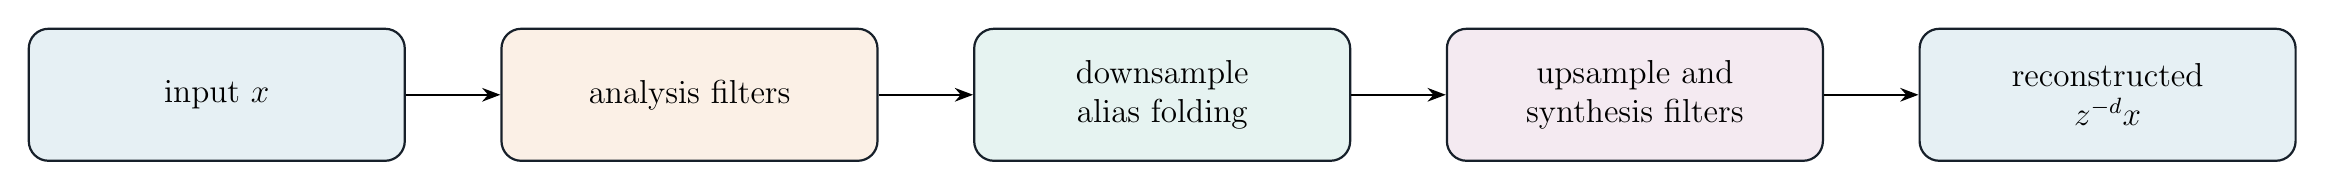
\begin{tikzpicture}[>=Stealth,node distance=8mm and 12mm,
 box/.style={rounded corners=2.5mm,draw=Ink,thick,minimum width=1.88in,minimum height=.66in,align=center,font=\large}]
\node[box,fill=PaleBlue] (x) {input $x$};
\node[box,fill=PaleOrange,right=of x] (f) {analysis filters};
\node[box,fill=PaleTeal,right=of f] (d) {downsample\\alias folding};
\node[box,fill=PaleMagenta,right=of d] (u) {upsample and\\synthesis filters};
\node[box,fill=PaleBlue,right=of u] (r) {reconstructed\\$z^{-d}x$};
\draw[->,thick] (x)--(f); \draw[->,thick] (f)--(d); \draw[->,thick] (d)--(u); \draw[->,thick] (u)--(r);
\end{tikzpicture}
\end{center}
\vspace{0.18in}
\TwoBox{PaleOrange}{\textbf{What downsampling does.}\par It folds spectral addresses together. A single branch generally cannot distinguish the collided coordinates.}{PaleTeal}{\textbf{What a perfect-reconstruction bank does.}\par Multiple branches carry complementary alias terms whose synthesis matrices cancel exactly.}
\vspace{0.18in}
\[
\mathbf R(z)\mathbf E(z)=z^{-d}I
\qquad\Longleftrightarrow\qquad
\text{distortion control and alias cancellation in one operator identity.}
\]
\vfill
\Callout{Polyphase coordinates make the cancellation visible as matrix multiplication. Longer orthogonal wavelets and reversible lifting schemes change the factors, not the reconstruction grammar.}

\VisualPage[4.82in]{ALIASING}{Downsampling folds distinct Fourier addresses onto the same decimated coordinate}{51_alias_folding.pdf}{The tone at index $25$ becomes indistinguishable from index $-7$ after downsampling by two. This is the collision that a multichannel analysis bank must resolve.}

\VisualPage[4.82in]{ALIAS CANCELLATION}{The low and high Haar branches reconstruct only when both are synthesized}{52_haar_alias_cancellation.pdf}{Each decimated branch alone is incomplete. Their synthesized object-space contributions contain complementary terms whose sum exactly equals the input.}

\VisualPage[4.82in]{CONCRETE POLYPHASE BLOCKS}{A finite convolution becomes a numerical phase-to-phase matrix}{53_concrete_polyphase_matrix.pdf}{The four displayed blocks are the entries of $\mathcal A_2H\mathcal S_2$. Applying this block matrix in channel coordinates and interleaving gives the same output as direct convolution.}

\VisualPage[4.82in]{LONGER ORTHOGONAL WAVELETS}{The four-tap Daubechies bank satisfies the same perfect-reconstruction law}{54_daubechies2_filter_bank.pdf}{The low- and high-pass filters are power-complementary, and the finite periodic analysis matrix is orthogonal. Haar is therefore one simple member of a larger wavelet family available in the framework.}

\VisualPage[4.82in]{MULTILEVEL DAUBECHIES REFINEMENT}{Successive low-pass parents produce a hierarchy of detail children}{55_daubechies2_multilevel.pdf}{The approximation at level three and the three retained detail families synthesize the original signal exactly. No detail is “discarded” unless a later selector removes it.}

\VisualPage[4.82in]{REVERSIBLE LIFTING}{The CDF 5/3 transform can preserve integer data exactly}{56_reversible_cdf53_lifting.pdf}{Predict and update steps are triangular and explicitly invertible. With the displayed integer rounding rules, the transform returns every integer sample exactly.}

\VisualPage[4.82in]{GENERAL BRANCHING}{Refinement may be dyadic, ternary, or based on another address arity}{57_dyadic_vs_ternary_refinement.pdf}{The identity “parent equals the sum of all children” is independent of the branching factor. Dyadic wavelets are especially common, but the packet language itself is not restricted to base two.}

% Expanded Part VIII
\clearpage
\PageTitle[EXPANDED PART VIII]{Adaptive resolution, approximation, and failure diagnostics}
\begin{center}
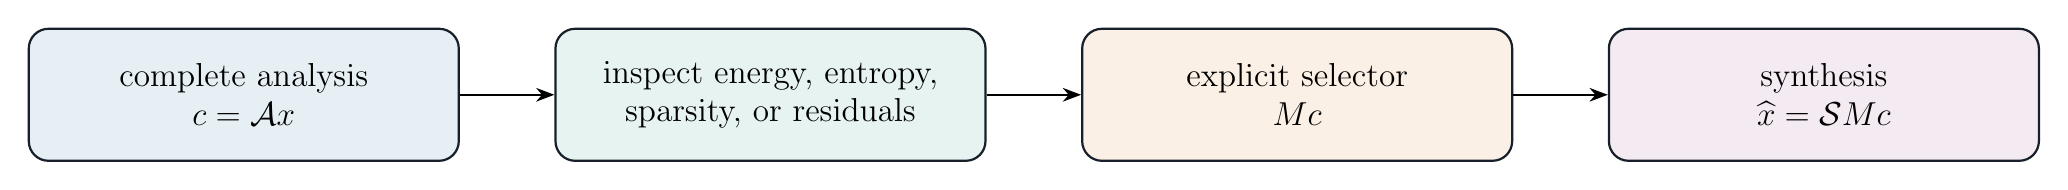
\begin{tikzpicture}[>=Stealth,node distance=7mm and 12mm,
 box/.style={rounded corners=2.5mm,draw=Ink,thick,minimum width=2.15in,minimum height=.66in,align=center,font=\large}]
\node[box,fill=PaleBlue] (a) {complete analysis\\$c=\mathcal Ax$};
\node[box,fill=PaleTeal,right=of a] (inspect) {inspect energy, entropy,\\sparsity, or residuals};
\node[box,fill=PaleOrange,right=of inspect] (m) {explicit selector\\$Mc$};
\node[box,fill=PaleMagenta,right=of m] (s) {synthesis\\$\widehat x=\mathcal S Mc$};
\draw[->,thick] (a)--(inspect); \draw[->,thick] (inspect)--(m); \draw[->,thick] (m)--(s);
\end{tikzpicture}
\end{center}
\vspace{0.18in}
\TwoBox{PaleTeal}{\textbf{Adaptive exact coordinates.}\par A best-basis algorithm may choose a mixed-depth complete leaf set and still reconstruct exactly.}{PaleOrange}{\textbf{Adaptive approximation.}\par Denoising, thresholding, sparse retention, and packet omission deliberately modify the complete coordinate tuple.}
\vspace{0.16in}
\[
r=x-\widehat x
\]
\begin{center}
The residual is not an afterthought: it identifies exactly what the selected coordinate system and synthesis failed to return.
\end{center}
\vfill
\Callout[PaleMagenta]{The next examples distinguish three separate decisions: where to stop refining, which coefficients to keep, and whether the synthesis operator still inverts the declared analysis.}

\VisualPage[4.82in]{MULTIRESOLUTION PYRAMID}{Every coarse approximation is accompanied by an exact detail ledger}{58_multiresolution_pyramid.pdf}{The signal is repeatedly split into a coarser parent and a detail child. Reversing the sequence with every detail present reconstructs the level-zero object exactly.}

\VisualPage[4.82in]{BEST-BASIS REFINEMENT}{Entropy chooses a mixed-depth complete wavelet-packet leaf set}{59_wavelet_packet_best_basis.pdf}{The selected leaves stop at different depths. They nevertheless form a complete pruned tree, so synthesis remains exact; adaptivity changes the coordinate partition, not the represented object.}

\VisualPage[4.82in]{DENOISING}{Thresholding is an explicit nonlinear selector after complete analysis}{60_wavelet_denoising_pipeline.pdf}{The wavelet transform itself is exactly invertible. The improved denoising error comes from deleting or shrinking coordinates, so the result is correctly labeled an approximation rather than perfect reconstruction.}

\VisualPage[4.82in]{OMITTED PACKET}{Dropping one packet makes the residual equal that packet}{61_missing_packet_diagnostic.pdf}{For a complete orthogonal packet family, synthesizing all but one packet gives $x-Q_\gamma x$. The residual is therefore exactly $Q_\gamma x$, providing a localized certificate of missing information.}

\VisualPage[4.82in]{SYNTHESIS MISMATCH}{A perturbed inverse breaks the perfect-reconstruction operator identity}{62_synthesis_mismatch.pdf}{Even when every analysis coefficient is retained, an incompatible synthesis bank produces $RE\ne I$. The matrix residual and object residual increase with the perturbation scale.}

\VisualPage[4.82in]{COEFFICIENT CONCENTRATION}{A signal zoo reveals which atlas makes a structure sparse}{63_signal_zoo_concentration.pdf}{Smooth periodic data concentrates rapidly in Fourier coordinates, while localized and discontinuous structures may concentrate more rapidly in wavelet packets. No universal ordering is asserted.}

\VisualPage[4.82in]{RATE--DISTORTION}{Equal coefficient budgets lead to atlas-dependent approximation errors}{64_signal_zoo_rate_distortion.pdf}{Both transforms are exact when all coefficients are kept. Their errors separate only after a largest-coefficient selector imposes the same finite budget.}

% Expanded Part IX
\clearpage
\PageTitle[EXPANDED PART IX]{Operator simplicity and nonlinear packet interactions}
\begin{minipage}[t]{0.47\linewidth}
\colorbox{PaleBlue}{\parbox{0.94\linewidth}{
\vspace{7pt}
\textbf{Linear transfer blocks}
\[
T=\sum_{\alpha,\beta}P_\beta TP_\alpha.
\]
A good atlas may make this block matrix diagonal, banded, sparse, local, or multiscale.
\vspace{6pt}}}
\end{minipage}\hfill
\begin{minipage}[t]{0.47\linewidth}
\colorbox{PaleOrange}{\parbox{0.94\linewidth}{
\vspace{7pt}
\textbf{Quadratic interaction packets}
\[
\mathcal N\!\left(\sum_\alpha x_\alpha\right)
=\sum_{\alpha,\beta}\mathcal N_{\alpha\beta}(x_\alpha,x_\beta).
\]
Nonlinear maps require self- and cross-packet terms rather than a single transfer matrix.
\vspace{6pt}}}
\end{minipage}
\vspace{0.20in}
\begin{center}
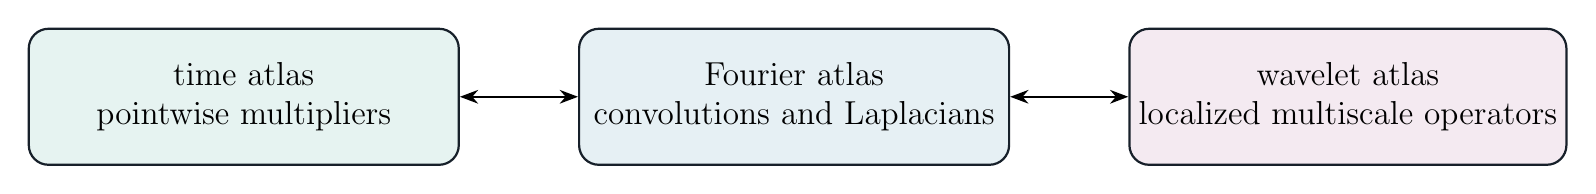
\begin{tikzpicture}[>=Stealth,node distance=10mm and 15mm,
 box/.style={rounded corners=2.5mm,draw=Ink,thick,minimum width=2.15in,minimum height=.68in,align=center,font=\large}]
\node[box,fill=PaleTeal] (time) {time atlas\\pointwise multipliers};
\node[box,fill=PaleBlue,right=of time] (four) {Fourier atlas\\convolutions and Laplacians};
\node[box,fill=PaleMagenta,right=of four] (wave) {wavelet atlas\\localized multiscale operators};
\draw[<->,thick] (time)--(four); \draw[<->,thick] (four)--(wave);
\end{tikzpicture}
\end{center}
\vfill
\Callout{The object does not change when the atlas changes, but the apparent complexity of its operator can change dramatically. Nonlinear examples add another layer: packet pairs may create new output addresses.}

\VisualPage[4.82in]{NATURAL OPERATOR ATLASES}{Different operators become diagonal in different coordinate systems}{65_operator_sparsity_by_atlas.pdf}{A spatial multiplier is simplest in time coordinates, circular convolution in Fourier coordinates, and a wavelet-packet projector in its own wavelet coordinates. Atlas choice is therefore also operator choice.}

\VisualPage[4.82in]{DIFFERENTIAL OPERATORS}{The periodic Laplacian is local in space and diagonal in Fourier space}{66_laplacian_in_three_atlases.pdf}{The wavelet representation exposes multiscale couplings instead. These are three coordinate views of the same operator, related by exact conjugation.}

\VisualPage[4.82in]{CONVOLUTION THEOREM}{Fourier coordinates turn circular convolution into coordinatewise multiplication}{67_convolution_theorem.pdf}{The spectral identity $F(h*x)=(Fh)(Fx)$ is the statement that the convolution operator is diagonal in the Fourier atlas. The plotted residual certifies the two computational routes agree.}

\VisualPage[4.82in]{QUADRATIC DECOMPOSITION}{A square contains two self-interactions and one cross-interaction}{68_quadratic_packet_interactions.pdf}{For $x=a+b$, exact nonlinear reconstruction requires $a^2$, $2ab$, and $b^2$. Omitting the cross term would lose information even though the original linear packet decomposition was complete.}

\VisualPage[4.82in]{FREQUENCY MIXING}{Multiplying two Fourier packets creates sum and difference addresses}{69_frequency_mixing.pdf}{The product of tones at frequencies $f_1$ and $f_2$ contains packets at $|f_2-f_1|$ and $f_1+f_2$. Nonlinear transfer therefore changes the packet address set.}

\VisualPage[4.82in]{INTERACTION HYPERGRAPH}{A quadratic map is resolved by input-pair to output-packet couplings}{70_nonlinear_interaction_hypergraph.pdf}{Each heatmap is one output slice of a three-index interaction tensor. It records how strongly every pair of input frequency packets contributes to a selected output band.}

\VisualPage[4.82in]{PRACTICAL NAVIGATION}{Choose an atlas by the structure and operator you need to expose}{71_atlas_selection_map.pdf}{The decision map is heuristic, not a theorem. It summarizes common starting points while preserving the requirement that the chosen analysis, selection, and synthesis operators be declared and tested.}


\VisualPage[4.82in]{EXPANDED CERTIFICATES}{The new exact examples are accompanied by numerical residuals}{72_extended_verification_dashboard.pdf}{Values near machine precision certify the implemented finite identities. The deliberately nonzero commutator is a compatibility diagnostic and is not presented as a failed reconstruction.}

% Advanced continuation map
\clearpage
\PageTitle[COMPREHENSIVE CONTINUATION]{Six further routes through the same reconstruction grammar}
\begin{center}
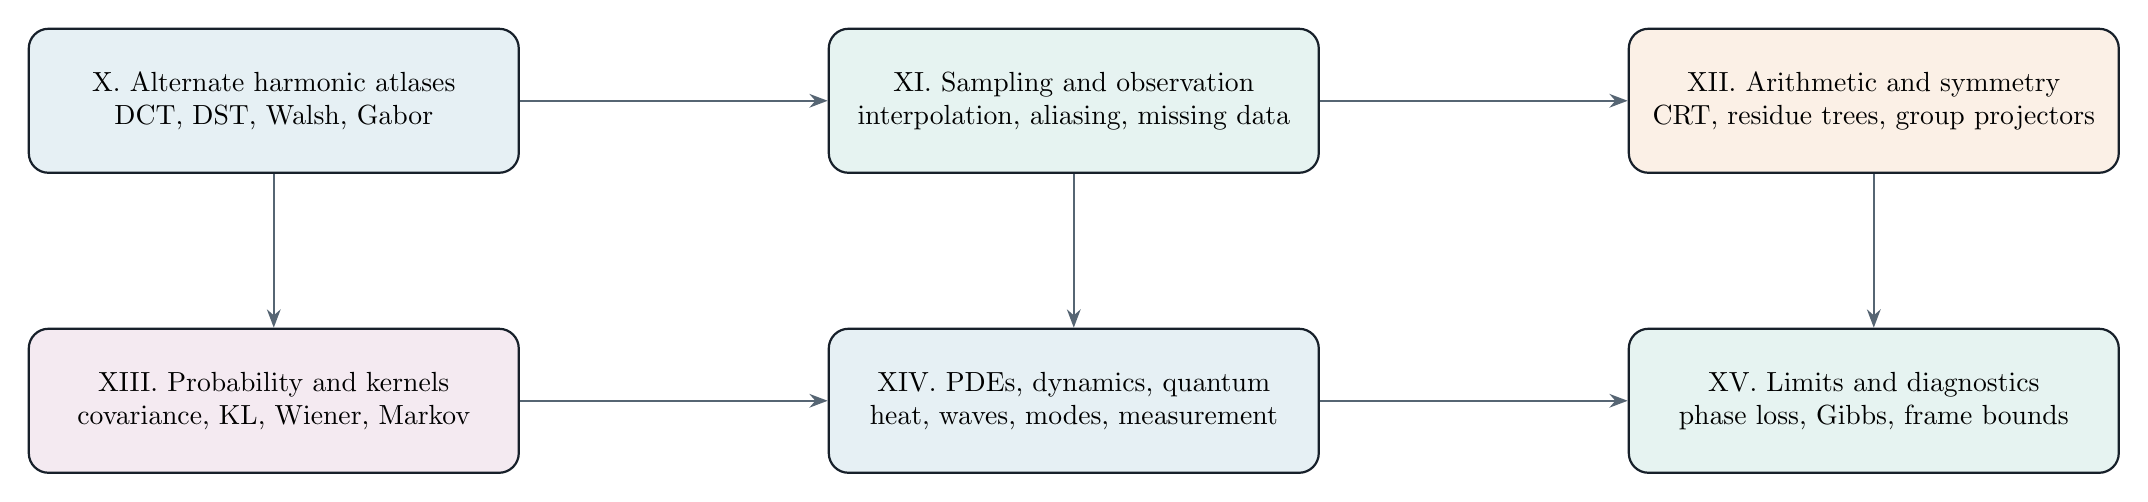
\begin{tikzpicture}[x=1in,y=1in,>=Stealth,
 box/.style={rounded corners=2.5mm,draw=Ink,thick,minimum width=2.45in,minimum height=.72in,align=center,font=\normalsize},
 arr/.style={->,thick,draw=Muted}]
\node[box,fill=PaleBlue] at (0,1.65) (harm) {X. Alternate harmonic atlases\\DCT, DST, Walsh, Gabor};
\node[box,fill=PaleTeal] at (4.0,1.65) (sample) {XI. Sampling and observation\\interpolation, aliasing, missing data};
\node[box,fill=PaleOrange] at (8.0,1.65) (arith) {XII. Arithmetic and symmetry\\CRT, residue trees, group projectors};
\node[box,fill=PaleMagenta] at (0,.15) (prob) {XIII. Probability and kernels\\covariance, KL, Wiener, Markov};
\node[box,fill=PaleBlue] at (4.0,.15) (pde) {XIV. PDEs, dynamics, quantum\\heat, waves, modes, measurement};
\node[box,fill=PaleTeal] at (8.0,.15) (limits) {XV. Limits and diagnostics\\phase loss, Gibbs, frame bounds};
\draw[arr] (harm)--(sample); \draw[arr] (sample)--(arith);
\draw[arr] (harm)--(prob); \draw[arr] (sample)--(pde); \draw[arr] (arith)--(limits);
\draw[arr] (prob)--(pde); \draw[arr] (pde)--(limits);
\end{tikzpicture}
\end{center}
\vspace{0.16in}
\TwoBox{PaleTeal}{\textbf{The exact rule does not change.}\par Each new construction identifies an analysis map, its coordinate packets or frame vectors, and a compatible synthesis.}{PaleOrange}{\textbf{The new boundary questions do change.}\par Sampling may fail to be injective, phase may be omitted, statistical filters may be deliberately lossy, and stable inversion may require frame or conditioning bounds.}
\vfill
\Callout[PaleMagenta]{The additional examples are not presented as newly invented transforms. They show how established harmonic, sampling, group, probabilistic, dynamical, and quantum constructions can be read inside the same declared analysis--transfer--selection--synthesis language.}

% Comprehensive Part X
\clearpage
\PageTitle[COMPREHENSIVE PART X]{Alternate harmonic coordinates and boundary-aware atlases}
\begin{minipage}[t]{0.47\linewidth}
\colorbox{PaleBlue}{\parbox{0.94\linewidth}{
\vspace{7pt}
\textbf{Boundary conditions are part of the atlas.}
\[
C^TC=I,\qquad S^TS=I,\qquad H^TH=I.
\]
Cosine, sine, and Walsh transforms differ in their atoms and implied extensions, not in the requirement of complete synthesis.
\vspace{6pt}}}
\end{minipage}\hfill
\begin{minipage}[t]{0.47\linewidth}
\colorbox{PaleTeal}{\parbox{0.94\linewidth}{
\vspace{7pt}
\textbf{Redundant time--frequency coordinates.}
\[
\mathcal S\mathcal A=I
\]
may hold even when the coefficient space is larger than the object space. The canonical dual inverts the frame operator.
\vspace{6pt}}}
\end{minipage}
\vspace{0.20in}
\begin{center}
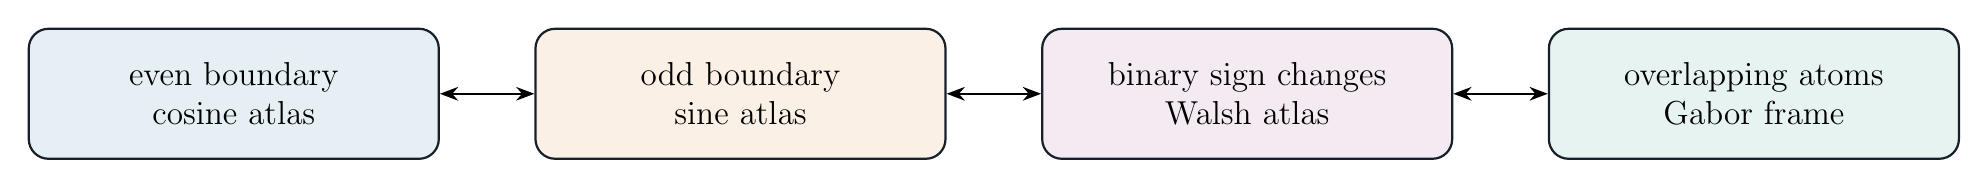
\begin{tikzpicture}[>=Stealth,node distance=8mm and 12mm,
 box/.style={rounded corners=2.5mm,draw=Ink,thick,minimum width=2.05in,minimum height=.65in,align=center,font=\large}]
\node[box,fill=PaleBlue] (dct) {even boundary\\cosine atlas};
\node[box,fill=PaleOrange,right=of dct] (dst) {odd boundary\\sine atlas};
\node[box,fill=PaleMagenta,right=of dst] (walsh) {binary sign changes\\Walsh atlas};
\node[box,fill=PaleTeal,right=of walsh] (gabor) {overlapping atoms\\Gabor frame};
\draw[<->,thick] (dct)--(dst); \draw[<->,thick] (dst)--(walsh); \draw[<->,thick] (walsh)--(gabor);
\end{tikzpicture}
\end{center}
\vfill
\Callout{These atlases are useful precisely because a complete coordinate system need not look sinusoidal, global, nonredundant, or periodic.}

\VisualPage[4.82in]{COSINE ATLAS}{An even extension produces exact boundary-aware cosine coordinates}{73_dct_even_extension.pdf}{The orthonormal DCT-II is a complete transform atlas. Its even-extension interpretation makes it natural for finite data whose endpoints should not be identified periodically.}

\VisualPage[4.82in]{SINE ATLAS}{An odd extension produces exact sine coordinates with zero boundaries}{74_dst_odd_extension.pdf}{The DST-I uses sine atoms adapted to implicit zero endpoints. Keeping every coordinate and applying the transpose reconstructs the interior data to floating-point precision.}

\VisualPage[4.82in]{WALSH ATLAS}{Binary sign-change atoms replace sinusoidal oscillations}{75_walsh_hadamard_atlas.pdf}{The sequency-ordered Walsh--Hadamard transform is orthogonal and exact. Piecewise-constant structure may concentrate naturally in this non-sinusoidal harmonic atlas.}

\VisualPage[4.82in]{BLOCK COORDINATES}{A block address and a local cosine index form a tensor-product packet}{76_block_dct_packets.pdf}{The complete block DCT reconstructs exactly. Keeping only a few local cosine coordinates per block is a later compression selector and therefore has a reported residual.}

\VisualPage[4.82in]{REDUNDANT GABOR FRAME}{Overlapping time--frequency atoms reconstruct through a canonical dual}{77_gabor_frame_dual_synthesis.pdf}{The analysis has more coordinates than the signal dimension. Exact synthesis is nevertheless possible because the frame operator is invertible and the displayed dual satisfies $\mathcal S\mathcal A=I$.}

\VisualPage[4.82in]{UNCERTAINTY AND CONCENTRATION}{No single atlas concentrates every object equally}{78_time_frequency_uncertainty.pdf}{An impulse, tone, Gaussian pulse, and chirp occupy time and frequency coordinates differently. This is a structural tradeoff, not a failure of either complete atlas.}

% Comprehensive Part XI
\clearpage
\PageTitle[COMPREHENSIVE PART XI]{Sampling, interpolation, and incomplete observation}
\begin{center}
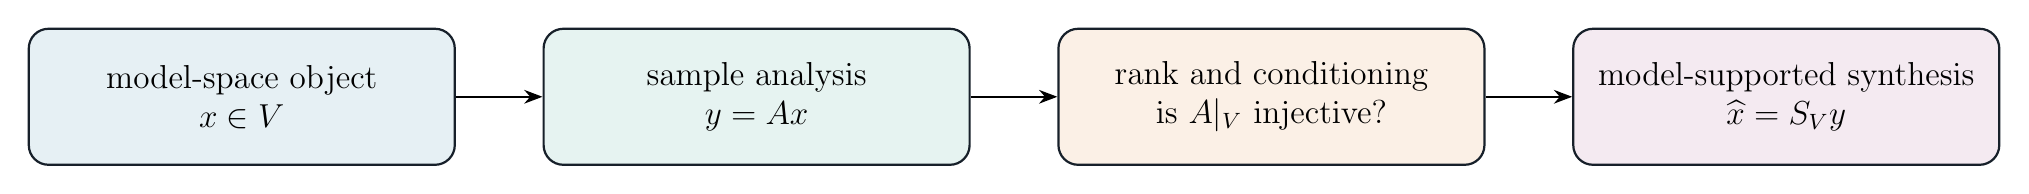
\begin{tikzpicture}[>=Stealth,node distance=8mm and 11mm,
 box/.style={rounded corners=2.5mm,draw=Ink,thick,minimum width=2.13in,minimum height=.68in,align=center,font=\large}]
\node[box,fill=PaleBlue] (x) {model-space object\\$x\in V$};
\node[box,fill=PaleTeal,right=of x] (a) {sample analysis\\$y=Ax$};
\node[box,fill=PaleOrange,right=of a] (rank) {rank and conditioning\\is $A|_V$ injective?};
\node[box,fill=PaleMagenta,right=of rank] (s) {model-supported synthesis\\$\widehat x=S_Vy$};
\draw[->,thick] (x)--(a); \draw[->,thick] (a)--(rank); \draw[->,thick] (rank)--(s);
\end{tikzpicture}
\end{center}
\vspace{0.17in}
\TwoBox{PaleTeal}{\textbf{Exact interpolation.}\par A finite bandlimited model and a full-rank sampling matrix can turn sparse or irregular observations into exact coordinates on that model space.}{PaleOrange}{\textbf{Aliasing or instability.}\par Too few samples destroy injectivity; clustered samples may preserve injectivity but amplify perturbations.}
\vfill
\Callout{Samples alone do not determine an arbitrary object. Exact recovery statements always include the declared finite model space, sampling map, and conditioning assumptions.}

\VisualPage[4.82in]{BANDLIMITED INTERPOLATION}{A complete finite mode model can be reconstructed from samples}{79_bandlimited_interpolation.pdf}{The sample values determine the displayed trigonometric polynomial because the sampling matrix has full column rank on the declared mode set. The reconstruction residual is near machine precision.}

\VisualPage[4.82in]{ALIASING}{Undersampling identifies distinct frequency packets}{80_aliasing_collision.pdf}{The two continuous tones differ between samples but agree at every sampled address. Their sampled coordinate tuple is therefore noninjective, which is exactly what aliasing means.}

\VisualPage[4.82in]{NONUNIFORM SAMPLING}{Irregular addresses can still form an exact finite analysis map}{81_nonuniform_fourier_reconstruction.pdf}{Uniform spacing is not required. Full column rank of the nonuniform Fourier design matrix is enough for exact synthesis on the chosen mode space.}

\VisualPage[4.82in]{SAMPLING CONDITIONING}{Completeness can survive while stability deteriorates}{82_sampling_conditioning.pdf}{As sample addresses cluster, the analysis matrix remains invertible over much of the path but its condition number and coefficient-noise amplification grow sharply.}

\VisualPage[4.82in]{MISSING COORDINATES}{A declared bandlimit can support exact recovery from a sampling mask}{83_missing_sample_recovery.pdf}{The hidden samples are not recovered from the mask alone. They are reconstructed because the object is assumed to lie in a finite Fourier mode space and enough observed addresses remain.}

\VisualPage[4.82in]{OVERLAP--ADD}{Window packets reconstruct when their synthesis weights form a partition of unity}{84_cola_window_packets.pdf}{The overlapping periodic Hann windows sum to one. Their windowed packet contributions therefore synthesize the original signal exactly despite substantial coordinate overlap.}

% Comprehensive Part XII
\clearpage
\PageTitle[COMPREHENSIVE PART XII]{Arithmetic addresses, residue refinement, and symmetry projectors}
\begin{minipage}[t]{0.47\linewidth}
\colorbox{PaleOrange}{\parbox{0.94\linewidth}{
\vspace{7pt}
\textbf{Arithmetic packet labels}
\[
n\longmapsto (n\bmod m_1,\ldots,n\bmod m_r)
\]
can refine a single residue address into compatible mixed-radix coordinates.
\vspace{6pt}}}
\end{minipage}\hfill
\begin{minipage}[t]{0.47\linewidth}
\colorbox{PaleMagenta}{\parbox{0.94\linewidth}{
\vspace{7pt}
\textbf{Symmetry packet labels}
\[
P_{\mathrm{inv}}=\frac1{|G|}\sum_{g\in G}\rho(g)
\]
select the group-invariant component; complementary packets record the broken symmetry.
\vspace{6pt}}}
\end{minipage}
\vspace{0.22in}
\begin{center}
\Large
Arithmetic refinement and group averaging are two different ways to manufacture exact projector families from structure already present in the object space.
\end{center}
\vfill
\Callout[PaleTeal]{The binary and ternary residue trees are finite visual models of hierarchical address refinement. They do not by themselves assert unrestricted $p$-adic analytic completion.}

\VisualPage[4.82in]{CHINESE REMAINDER COORDINATES}{Residues modulo two and three identify the same packet as a residue modulo six}{85_chinese_remainder_packets.pdf}{The coprime coordinate pair gives a bijective label for the six residue packets. Summing all six object-space packets reconstructs the signal exactly.}

\VisualPage[4.82in]{MIXED-RADIX POLYPHASE}{A residue modulo twelve can be addressed simultaneously modulo three and four}{86_mixed_radix_polyphase.pdf}{The phase lattice displays a two-coordinate label for each modulo-twelve channel. This is an address refinement, not a change to the underlying samples.}

\VisualPage[4.82in]{DYADIC RESIDUE TREE}{Every binary parent packet is the exact sum of two children}{87_dyadic_residue_tree.pdf}{The node values show packet energies while the edges encode $P_{2^j,r}=P_{2^{j+1},r}+P_{2^{j+1},r+2^j}$. The refinement residual is exactly zero in the finite model.}

\VisualPage[4.82in]{TERNARY RESIDUE TREE}{The same refinement law holds with three children per parent}{88_ternary_residue_tree.pdf}{Nonbinary refinement obeys the same completeness rule. Each modulo-$3^j$ packet is exactly synthesized from its three modulo-$3^{j+1}$ children.}

\VisualPage[4.82in]{GROUP-AVERAGING PROJECTOR}{Averaging over the dihedral group selects the invariant image packet}{89_dihedral_group_projector.pdf}{Applying the group average twice changes nothing, and the original image is the exact sum of its invariant packet and noninvariant residual.}

\VisualPage[4.82in]{TENSOR SYMMETRY}{Swap symmetry splits a matrix into symmetric and antisymmetric packets}{90_symmetric_antisymmetric_packets.pdf}{The projectors $P_\pm(X)=\frac12(X\pm X^T)$ are complementary and exact. They provide a simple tensor-valued example of symmetry-resolved decomposition.}

% Comprehensive Part XIII
\clearpage
\PageTitle[COMPREHENSIVE PART XIII]{Probability, covariance, stochastic transfer, and kernel coordinates}
\begin{center}
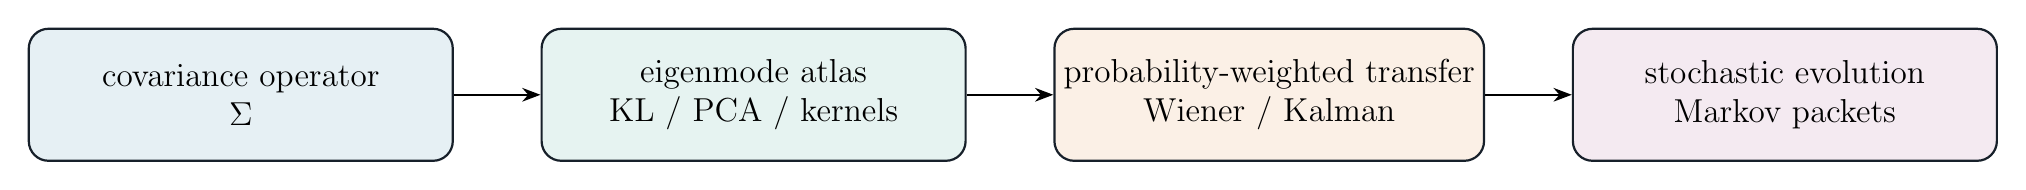
\begin{tikzpicture}[>=Stealth,node distance=8mm and 11mm,
 box/.style={rounded corners=2.5mm,draw=Ink,thick,minimum width=2.12in,minimum height=.66in,align=center,font=\large}]
\node[box,fill=PaleBlue] (cov) {covariance operator\\$\Sigma$};
\node[box,fill=PaleTeal,right=of cov] (modes) {eigenmode atlas\\KL / PCA / kernels};
\node[box,fill=PaleOrange,right=of modes] (transfer) {probability-weighted transfer\\Wiener / Kalman};
\node[box,fill=PaleMagenta,right=of transfer] (dyn) {stochastic evolution\\Markov packets};
\draw[->,thick] (cov)--(modes); \draw[->,thick] (modes)--(transfer); \draw[->,thick] (transfer)--(dyn);
\end{tikzpicture}
\end{center}
\vspace{0.18in}
\TwoBox{PaleTeal}{\textbf{Exact coordinate statements.}\par Covariance, kernel, and Markov operators admit complete finite spectral decompositions, and all modes synthesize exactly.}{PaleOrange}{\textbf{Statistical decisions.}\par Wiener filtering and Bayesian updating weight coordinates by uncertainty; they are not perfect-reconstruction claims about the unknown noise-free object.}
\vfill
\Callout{Probability changes the interpretation of the transfer blocks and selectors, but the bookkeeping remains explicit: operator, coordinates, weights, synthesis, and residual.}

\VisualPage[4.82in]{COVARIANCE BLOCKS}{A covariance operator decomposes into packet-to-packet dependence blocks}{91_covariance_transfer_blocks.pdf}{Variable-group projectors expose within-group and cross-group covariance. Summing the nine displayed blocks reconstructs the covariance matrix exactly.}

\VisualPage[4.82in]{KARHUNEN--LOEVE ATLAS}{Covariance eigenvectors adapt coordinates to an ensemble}{92_karhunen_loeve_atlas.pdf}{All empirical eigenmodes reconstruct each centered realization exactly. Retaining only the leading modes is a variance-based approximation with a separately reported error.}

\VisualPage[4.82in]{WIENER TRANSFER}{Signal-to-noise weights act as spectral transfer multipliers}{93_wiener_spectral_transfer.pdf}{The filter downweights frequency packets estimated to be noise-dominated. The improved RMSE is a statistical approximation result, not a perfect-reconstruction certificate.}

\VisualPage[4.82in]{MARKOV PACKETS}{A reversible transition operator separates stationary and transient modes}{94_markov_spectral_packets.pdf}{The leading eigenpacket is stationary while the remaining packets decay by powers of their eigenvalues. Their complete spectral sum matches direct matrix evolution.}

\VisualPage[4.82in]{KALMAN UPDATE}{Measurement innovation is transferred into the state by a covariance-weighted gain}{95_kalman_update_geometry.pdf}{The posterior mean is the prior plus a gain-weighted innovation, while the posterior covariance contracts most strongly in the observed direction.}

\VisualPage[4.82in]{KERNEL EIGENFUNCTIONS}{A positive kernel supplies another geometry-dependent spectral atlas}{96_kernel_eigen_atlas.pdf}{All kernel eigenvectors synthesize the finite object exactly. Truncating to the leading kernel coordinates creates a smooth low-rank approximation whose residual is reported.}

% Comprehensive Part XIV
\clearpage
\PageTitle[COMPREHENSIVE PART XIV]{PDEs, dynamical modes, and quantum coordinates}
\begin{minipage}[t]{0.47\linewidth}
\colorbox{PaleBlue}{\parbox{0.94\linewidth}{
\vspace{7pt}
\textbf{Linear evolution in a diagonal atlas}
\[
x(t)=U^{-1}\operatorname{diag}(g_k(t))Ux(0).
\]
Each spectral packet evolves by its own scalar law before exact synthesis.
\vspace{6pt}}}
\end{minipage}\hfill
\begin{minipage}[t]{0.47\linewidth}
\colorbox{PaleMagenta}{\parbox{0.94\linewidth}{
\vspace{7pt}
\textbf{Quantum coordinates}
\[
\psi=\sum_jP_j\psi,\qquad p_j=\|P_j\psi\|^2.
\]
Coherent packet synthesis is exact; selecting a measurement outcome is not reversible.
\vspace{6pt}}}
\end{minipage}
\vspace{0.22in}
\begin{center}
\Large
Heat decay, wave propagation, Poisson inversion, normal modes, data-driven dynamics, and quantum basis changes all become coordinatewise transfer once a suitable atlas is declared.
\end{center}
\vfill
\Callout[PaleOrange]{These are finite discretizations and finite-dimensional state examples. They visualize the operator grammar without claiming that every infinite-dimensional domain issue has disappeared.}

\VisualPage[4.82in]{HEAT SEMIGROUP}{Diffusive evolution multiplies every Fourier packet by a decaying scalar}{97_heat_equation_spectral_decay.pdf}{Higher-frequency packets decay faster. The spectral synthesis at the final time agrees with a direct matrix-exponential computation to floating-point precision.}

\VisualPage[4.82in]{WAVE EQUATION}{Independent oscillatory packets synthesize a propagating finite wave}{98_wave_equation_modal_reconstruction.pdf}{Each Laplacian eigenpacket oscillates at its modal frequency. Their complete sum produces the displayed motion while the finite modal energy remains constant.}

\VisualPage[4.82in]{POISSON SOLVER}{A periodic elliptic inverse divides nonconstant spectral packets by their eigenvalues}{99_poisson_spectral_solver.pdf}{The constant packet is excluded by the zero-mean condition. The reconstructed solution satisfies the discrete Poisson equation with a residual near numerical precision.}

\VisualPage[4.82in]{NORMAL MODES}{Coupled oscillators decouple in an eigenvector atlas}{100_coupled_oscillator_modes.pdf}{The initial displacement is analyzed into normal-mode coordinates, each coordinate evolves independently, and the physical displacement is synthesized from every mode.}

\VisualPage[4.82in]{DYNAMIC MODE DECOMPOSITION}{Observed trajectories can define a data-driven modal atlas}{101_dynamic_mode_decomposition.pdf}{For this exact linear example, DMD recovers the rotating-decaying eigenvalues and reconstructs the complete trajectory to floating-point precision.}

\VisualPage[4.82in]{QUANTUM MEASUREMENT}{Basis projectors decompose amplitudes and generate outcome probabilities}{102_quantum_measurement_packets.pdf}{The coherent sum of all projected amplitude packets is exactly the original state. Conditioning on one observed outcome discards the other coherent packets and is therefore not invertible.}

\VisualPage[4.82in]{QUANTUM FOURIER ATLAS}{The Fourier transform transports quantum amplitudes between address and character coordinates}{103_quantum_fourier_atlas.pdf}{An address-localized state spreads uniformly across Fourier outcomes, while a phase-ramp character concentrates into one frequency packet. The transform remains unitary and exactly invertible.}

% Comprehensive Part XV
\clearpage
\PageTitle[COMPREHENSIVE PART XV]{Limits, stability, model-based components, and multi-axis coordinates}
\begin{center}
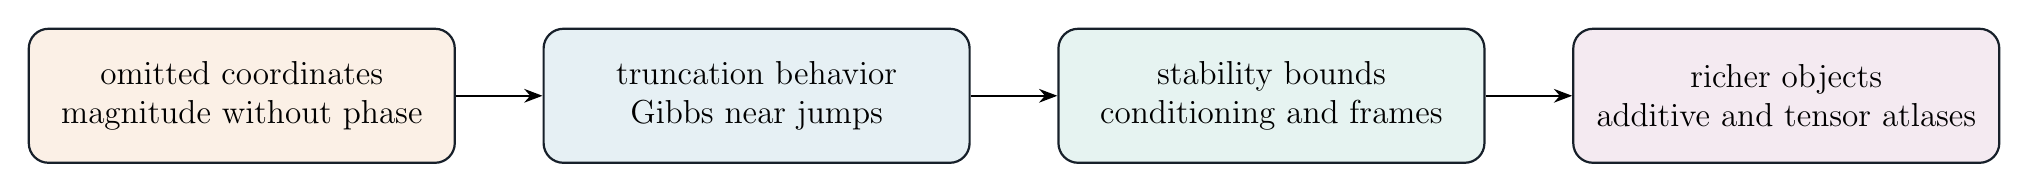
\begin{tikzpicture}[>=Stealth,node distance=8mm and 11mm,
 box/.style={rounded corners=2.5mm,draw=Ink,thick,minimum width=2.13in,minimum height=.67in,align=center,font=\large}]
\node[box,fill=PaleOrange] (omit) {omitted coordinates\\magnitude without phase};
\node[box,fill=PaleBlue,right=of omit] (truncate) {truncation behavior\\Gibbs near jumps};
\node[box,fill=PaleTeal,right=of truncate] (stable) {stability bounds\\conditioning and frames};
\node[box,fill=PaleMagenta,right=of stable] (multi) {richer objects\\additive and tensor atlases};
\draw[->,thick] (omit)--(truncate); \draw[->,thick] (truncate)--(stable); \draw[->,thick] (stable)--(multi);
\end{tikzpicture}
\end{center}
\vspace{0.17in}
\TwoBox{PaleOrange}{\textbf{A coordinate set may be incomplete.}\par Fourier magnitude without phase does not uniquely identify an object, even though the full complex Fourier transform is unitary.}{PaleTeal}{\textbf{An exact map may still be unstable.}\par Frame bounds and condition numbers control how coefficient perturbations propagate through synthesis.}
\vfill
\Callout{The final examples separate exact algebraic synthesis from injectivity, stability, compression behavior, and model-identifiability assumptions.}

\VisualPage[4.82in]{PHASE RETRIEVAL LIMIT}{Equal Fourier magnitudes can correspond to different objects}{104_phase_retrieval_ambiguity.pdf}{A circular shift preserves Fourier magnitude while changing phase and object location. Magnitude-only analysis is therefore incomplete even though the full Fourier atlas is exact.}

\VisualPage[4.82in]{GIBBS DIAGNOSTIC}{Oscillatory overshoot belongs to global Fourier truncation near a jump}{105_gibbs_and_local_packets.pdf}{The aligned local packet represents this dyadic step without ringing, while finite Fourier truncations overshoot. This is a comparison of approximations, not a claim that every wavelet approximation eliminates every boundary artifact.}

\VisualPage[4.82in]{FRAME STABILITY}{The lower frame bound controls sensitivity of dual synthesis}{106_frame_bounds_and_stability.pdf}{Every displayed frame remains exactly reconstructing in exact arithmetic, but coefficient-noise amplification grows when the frame operator becomes poorly conditioned.}

\VisualPage[4.82in]{MODEL-BASED ADDITIVE COMPONENTS}{Low-rank and sparse pieces may synthesize an object without being projector packets}{107_low_rank_sparse_components.pdf}{The sum is exact because the components were constructed additively. Identifying those components from the observed sum would require additional assumptions and an optimization or inference procedure.}

\VisualPage[4.82in]{MULTI-AXIS ATLAS}{Channel modes and temporal cosine modes can be resolved simultaneously}{108_multiaxis_channel_time_atlas.pdf}{A data-adapted channel transform and a DCT in time form a tensor-product atlas. The full coefficient matrix reconstructs every sensor sample exactly.}

\VisualPage[4.82in]{COMPREHENSIVE CERTIFICATES}{The additional exact identities and deliberate collisions are recorded together}{109_advanced_verification_dashboard.pdf}{Near-zero synthesis residuals verify the finite exact examples. Near-zero alias and phase-magnitude collisions intentionally certify noninjectivity of incomplete observations rather than successful object recovery.}

% Advanced quick reference
% Further-expanded route map
\clearpage
\PageTitle[CROSS-DOMAIN DEEPENING]{Five detailed cross-domain pathways through the same analysis--synthesis grammar}
\begin{center}
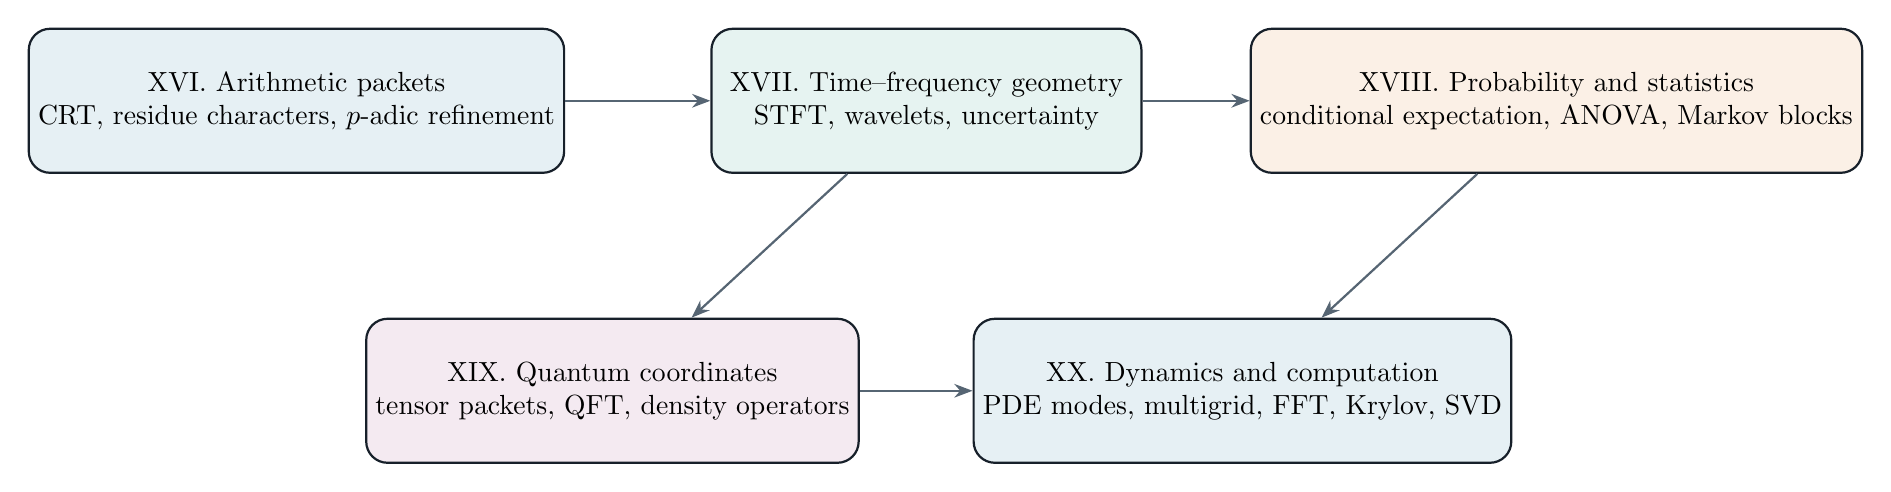
\begin{tikzpicture}[x=1in,y=1in,>=Stealth,
 box/.style={rounded corners=2.7mm,draw=Ink,thick,minimum width=2.15in,minimum height=.72in,align=center,font=\normalsize},
 arr/.style={->,thick,draw=Muted}]
\node[box,fill=PaleBlue] at (0,1.55) (arith) {XVI. Arithmetic packets\\CRT, residue characters, $p$-adic refinement};
\node[box,fill=PaleTeal] at (3.15,1.55) (tf) {XVII. Time--frequency geometry\\STFT, wavelets, uncertainty};
\node[box,fill=PaleOrange] at (6.30,1.55) (prob) {XVIII. Probability and statistics\\conditional expectation, ANOVA, Markov blocks};
\node[box,fill=PaleMagenta] at (1.58,.10) (quant) {XIX. Quantum coordinates\\tensor packets, QFT, density operators};
\node[box,fill=PaleBlue] at (4.73,.10) (pde) {XX. Dynamics and computation\\PDE modes, multigrid, FFT, Krylov, SVD};
\draw[arr] (arith)--(tf); \draw[arr] (tf)--(prob); \draw[arr] (tf)--(quant); \draw[arr] (prob)--(pde); \draw[arr] (quant)--(pde);
\end{tikzpicture}
\end{center}
\vspace{0.18in}
\TwoBox{PaleTeal}{\textbf{Same exact core.}\par Complete coordinate packets still synthesize the object, compatible transfer maps still connect resolutions, and every finite exact example is accompanied by a residual.}{PaleOrange}{\textbf{New domains, declared boundaries.}\par Classical harmonic, probabilistic, quantum, numerical, and algebraic constructions are visualized as realizations of the common grammar without claiming that those established constructions are newly invented.}
\vfill
\Callout[PaleMagenta]{The added pages are not an applications list. Each section isolates a specific structural bridge: residue refinement, local time--frequency tiling, conditional expectation, tensor-product quantum coordinates, or multilevel numerical correction.}

% Maximal Part XVI
\clearpage
\PageTitle[MAXIMAL PART XVI]{Arithmetic packets, congruence coordinates, and $p$-adic refinement}
\begin{minipage}[t]{0.47\linewidth}
\colorbox{PaleBlue}{\parbox{0.94\linewidth}{
\vspace{7pt}
\textbf{Additive residue packets}
\[
P_{m,r}=\frac1m\sum_{j=0}^{m-1}\omega^{-jr}U^j,
\qquad
\sum_{r=0}^{m-1}P_{m,r}=I.
\]
Roots of unity turn congruence selection into a finite spectral projector.
\vspace{5pt}}}
\end{minipage}\hfill
\begin{minipage}[t]{0.47\linewidth}
\colorbox{PaleOrange}{\parbox{0.94\linewidth}{
\vspace{7pt}
\textbf{Arithmetic refinement}
\[
P_{p^k,r}=\sum_{j=0}^{p-1}P_{p^{k+1},r+jp^k}.
\]
A $p$-adic address is a refinement path whose next digit selects one child packet.
\vspace{5pt}}}
\end{minipage}
\vspace{0.20in}
\begin{center}
\ClassicalBadge\qquad Chinese remainder coordinates, additive characters, multiplicative characters, and valuation shells are classical arithmetic structures represented in the common packet language.
\end{center}
\vfill
\Callout{This section makes the signal--arithmetic bridge explicit: polyphase residue channels, polynomial coefficient classes, congruence packets, and $p$-adic refinement are different realizations of address decomposition.}

\VisualPage[4.82in]{CHINESE REMAINDER COORDINATES}{One cyclic address can be resolved into compatible factor coordinates}{110_crt_coordinate_grid.pdf}{The Chinese remainder theorem identifies each address modulo 12 with one pair of addresses modulo 3 and modulo 4. The coordinate pair is exact because the moduli are coprime and every pair has one unique representative.}

\VisualPage[4.82in]{CRT PACKET SYNTHESIS}{Joint congruence packets reconstruct the full finite signal}{111_crt_signal_reconstruction.pdf}{The twelve joint packets are indexed by $(n\bmod 3,n\bmod 4)$ and are equivalent to the twelve residue packets modulo 12. Their disjoint sum reproduces every sample exactly.}

\VisualPage[4.82in]{$p$-ADIC REFINEMENT}{Binary and ternary address trees refine without changing the represented object}{112_p_adic_refinement_trees.pdf}{At level $k$, a packet fixes the first $k$ base-$p$ digits of an address. Retaining every child makes the refinement exact; the dyadic and ternary trees differ only in branching arity.}

\VisualPage[4.82in]{VALUATION SHELLS}{Divisibility depth creates a second arithmetic packet geometry}{113_valuation_shell_packets.pdf}{Residue packets classify an integer by its remainder, while valuation packets classify it by the largest power of $p$ dividing it. Both are exact finite partitions when the zero or terminal shell is declared separately.}

\VisualPage[4.82in]{CHARACTER PROJECTORS}{Roots of unity select one congruence class by coherent addition}{114_roots_of_unity_residue_projector.pdf}{On the selected residue class the character phases align; elsewhere they form a cancelling polygon. The resulting character average equals the ordinary residue mask to floating-point precision.}

\VisualPage[4.82in]{MULTIPLICATIVE CHARACTERS}{The unit group has its own finite Fourier coordinate atlas}{115_dirichlet_character_packets.pdf}{Characters of $\mathbb F_5^*$ analyze functions on the nonzero residues. The unitary character matrix reconstructs the function exactly, just as an additive DFT reconstructs a cyclic signal.}

\VisualPage[4.82in]{GAUSS-SUM TRANSFER}{Additive and multiplicative harmonic atlases are linked by structured blocks}{116_gauss_sum_transition.pdf}{Gauss sums measure the transition between additive-frequency and multiplicative-character coordinates. For the nontrivial characters in the finite example, the magnitudes equal $\sqrt p$ up to roundoff.}

\VisualPage[4.82in]{POLYNOMIAL POLYPHASE}{Coefficient degrees split into exact residue packets}{117_polynomial_residue_packets.pdf}{The identity $f(z)=f_0(z^3)+z f_1(z^3)+z^2f_2(z^3)$ is a polyphase decomposition of polynomial coefficients. It is the same residue-address logic used for sampled signals.}

% Maximal Part XVII
\clearpage
\PageTitle[MAXIMAL PART XVII]{Time--frequency localization and scale-dependent coordinates}
\begin{center}
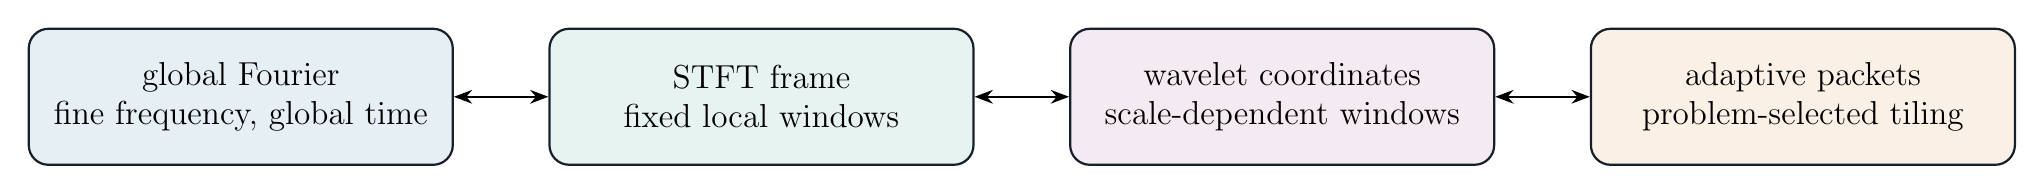
\begin{tikzpicture}[>=Stealth,node distance=8mm and 12mm,
 box/.style={rounded corners=2.5mm,draw=Ink,thick,minimum width=2.12in,minimum height=.68in,align=center,font=\large}]
\node[box,fill=PaleBlue] (f) {global Fourier\\fine frequency, global time};
\node[box,fill=PaleTeal,right=of f] (s) {STFT frame\\fixed local windows};
\node[box,fill=PaleMagenta,right=of s] (w) {wavelet coordinates\\scale-dependent windows};
\node[box,fill=PaleOrange,right=of w] (a) {adaptive packets\\problem-selected tiling};
\draw[<->,thick] (f)--(s); \draw[<->,thick] (s)--(w); \draw[<->,thick] (w)--(a);
\end{tikzpicture}
\end{center}
\vspace{0.20in}
\TwoBox{PaleTeal}{\textbf{Exact analysis--synthesis.}\par Global Fourier bases, complete wavelet bases, and compatible STFT frames all admit exact finite reconstruction.}{PaleOrange}{\textbf{Localization tradeoff.}\par Time and frequency concentration cannot both be arbitrarily sharp. Atlas design chooses how the available resolution is distributed.}
\vfill
\Callout{The following pages show the geometry behind “Fourier space and wavelets are both available”: they occupy different tilings of the same time--frequency plane and are connected by exact coordinate transforms or dual-frame synthesis.}

\VisualPage[4.82in]{TIME--FREQUENCY TILINGS}{Fourier, STFT, and wavelet atlases distribute resolution differently}{118_heisenberg_tilings.pdf}{Global Fourier bins span all times, STFT packets use a fixed grid of local rectangles, and wavelet packets use scale-dependent rectangles. The diagrams show coordinate geometry, not a claim that one tiling is universally best.}

\VisualPage[4.82in]{OVERLAP--ADD WINDOWS}{Shifted windows can form an exact partition of unity}{119_overlap_add_partition.pdf}{Periodic Hann windows with fifty-percent overlap sum to one at every sample. This pointwise identity is the simplest object-space certificate behind overlap--add synthesis.}

\VisualPage[4.82in]{DUAL STFT SYNTHESIS}{A redundant local-Fourier frame reconstructs through a compatible dual}{120_dual_window_stft_reconstruction.pdf}{The STFT analysis matrix contains more rows than the signal dimension. Exact recovery comes from the dual synthesis operator $A^{\dagger}$ and the frame identity $A^{\dagger}A=I$, not from a square basis matrix.}

\VisualPage[4.82in]{LOCAL FOURIER MOTION}{A spectrogram follows a chirp and a transient burst through time}{121_chirp_spectrogram.pdf}{The rising ridge records the chirp, while the compact high-frequency patch records the localized burst. Both structures are present in the global signal, but local Fourier packets make their timing visible.}

\VisualPage[4.82in]{WAVELET SCALOGRAM}{Morlet coordinates reveal the same signal with scale-dependent support}{122_morlet_scalogram.pdf}{Wavelet scales provide narrower time support at high pseudo-frequency and broader support at low pseudo-frequency. The finite scalogram is a sampled continuous-wavelet visualization rather than a separate reconstruction theorem.}

\VisualPage[4.82in]{CONSTANT-$Q$ PACKETS}{Equal relative bandwidth produces a logarithmic frequency geometry}{123_constant_q_tiling.pdf}{Constant-$Q$ packets devote long windows to low frequencies and short windows to high frequencies. This is another lawful time--frequency atlas, useful when ratios of frequency matter more than equal frequency increments.}

\VisualPage[4.82in]{ADAPTIVE FREQUENCY PARTITIONS}{Wavelet-packet leaves may stop at different depths}{124_wavelet_packet_frequency_tiling.pdf}{A uniform-depth packet tree gives equal-width terminal bands. A best-basis leaf set may mix depths while still covering the complete address domain exactly before any coefficient thresholding.}

\VisualPage[4.82in]{UNCERTAINTY TRADEOFF}{Sharper time localization necessarily broadens frequency support}{125_uncertainty_tradeoff.pdf}{The sampled Gaussian family approaches the familiar minimum spread product. The plot explains why Fourier, STFT, and wavelet packets cannot simultaneously use arbitrarily narrow time and frequency cells.}

% Maximal Part XVIII
\clearpage
\PageTitle[MAXIMAL PART XVIII]{Probability, statistics, and stochastic refinement}
\begin{minipage}[t]{0.47\linewidth}
\colorbox{PaleTeal}{\parbox{0.94\linewidth}{
\vspace{7pt}
\textbf{Projection in probability}
\[
E[X\mid\mathcal G]^2=E[X\mid\mathcal G]
\quad\text{as an operator on }L^2.
\]
In a finite model, conditional expectation averages within partition packets.
\vspace{5pt}}}
\end{minipage}\hfill
\begin{minipage}[t]{0.47\linewidth}
\colorbox{PaleOrange}{\parbox{0.94\linewidth}{
\vspace{7pt}
\textbf{Stochastic refinement}
\[
X=M_0+\sum_{k\ge1}(M_k-M_{k-1}).
\]
A filtration exposes progressively finer information, with increments recording what each refinement adds.
\vspace{5pt}}}
\end{minipage}
\vspace{0.18in}
\TwoBox{PaleBlue}{\textbf{Statistical packets.}\par ANOVA, least squares, PCA, whitening, and covariance modes separate mean, fitted structure, interactions, and residual components.}{PaleMagenta}{\textbf{Stochastic transfer.}\par A Markov chain closes on a coarse packet system only when state-level transition totals satisfy the appropriate lumpability condition.}
\vfill
\Callout{The examples remain finite and explicit. They show how projection, refinement, residuals, and block transfer appear in probability and statistics without replacing measure-theoretic domain conditions in the formal papers.}

\VisualPage[4.82in]{CONDITIONAL EXPECTATION}{A finite partition defines an orthogonal averaging projector}{126_conditional_expectation_projection.pdf}{The projected random variable is constant on each information block. The matrix is self-adjoint and idempotent under the uniform finite measure, so the discarded residual is orthogonal to every block-measurable coordinate.}

\VisualPage[4.82in]{FILTRATION REFINEMENT}{More information means a finer stochastic coordinate atlas}{127_filtration_refinement.pdf}{Each partition refines the previous one, and $M_k=E[X\mid\mathcal F_k]$ resolves more of the finite random variable. The final singleton partition returns the fully resolved object.}

\VisualPage[4.82in]{MARTINGALE INCREMENTS}{Refinement differences synthesize the final random variable}{128_martingale_increment_reconstruction.pdf}{The increments $D_k=M_k-M_{k-1}$ form a stochastic multiresolution ledger. Their sum with the coarsest expectation reconstructs the finite variable exactly.}

\VisualPage[4.82in]{ANOVA PACKETS}{Mean, main effects, and interactions form an exact table decomposition}{129_anova_decomposition.pdf}{The interaction packet has zero row and column means, while the grand mean and two main-effect families carry the lower-order structure. Summing all four components reconstructs the table.}

\VisualPage[4.82in]{LEAST-SQUARES GEOMETRY}{A fitted model is a projection and its residual is orthogonal}{130_least_squares_projection.pdf}{The hat matrix projects the observation vector onto the polynomial design space. The displayed residual satisfies $X^Tr\approx0$, giving a direct certificate that it lies outside the fitted coordinate subspace.}

\VisualPage[4.82in]{WHITENING}{Covariance-adapted coordinates turn ellipses into an identity metric}{131_whitening_atlas.pdf}{Eigenvector rotation and inverse-square-root scaling transform the declared covariance matrix to identity. The finite scatter shows sampling variation, while the operator-level covariance identity holds to roundoff.}

\VisualPage[4.82in]{MARKOV TRANSFER BLOCKS}{A lumpable chain closes exactly on a coarse state partition}{132_markov_transfer_blocks.pdf}{Every state within one source packet sends the same total probability into each target packet. The state-level chain therefore induces a well-defined packet-level transition matrix.}

\VisualPage[4.82in]{LUMPABILITY DIAGNOSTIC}{A small state-level perturbation can break coarse stochastic closure}{133_lumpability_diagnostic.pdf}{Moving probability between target packets makes the block totals depend on which state inside the source packet was chosen. The nonzero lumpability residual identifies that failure explicitly.}

% Maximal Part XVIIII
\clearpage
\PageTitle[MAXIMAL PART XIX]{Quantum bases, tensor packets, and density-operator coordinates}
\begin{center}
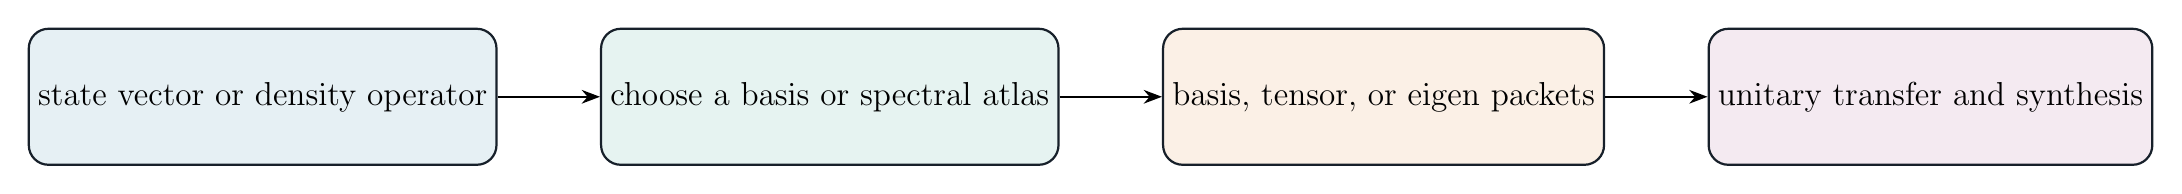
\begin{tikzpicture}[>=Stealth,node distance=8mm and 13mm,
 box/.style={rounded corners=2.5mm,draw=Ink,thick,minimum width=2.16in,minimum height=.68in,align=center,font=\large}]
\node[box,fill=PaleBlue] (state) {state vector or density operator};
\node[box,fill=PaleTeal,right=of state] (basis) {choose a basis or spectral atlas};
\node[box,fill=PaleOrange,right=of basis] (packets) {basis, tensor, or eigen packets};
\node[box,fill=PaleMagenta,right=of packets] (unitary) {unitary transfer and synthesis};
\draw[->,thick] (state)--(basis); \draw[->,thick] (basis)--(packets); \draw[->,thick] (packets)--(unitary);
\end{tikzpicture}
\end{center}
\vspace{0.18in}
\TwoBox{PaleTeal}{\textbf{Pure-state coordinates.}\par A normalized state decomposes in any orthonormal basis. Tensor-product projectors supply joint addresses for multipartite systems.}{PaleOrange}{\textbf{Density-operator coordinates.}\par A positive density matrix has an exact spectral decomposition; channels such as dephasing may preserve some packet families while suppressing others.}
\vfill
\Callout[PaleMagenta]{The quantum pages visualize coordinate decompositions and operator transfer only. A probability vector from one measurement basis is not treated as complete quantum-state tomography.}

\VisualPage[4.82in]{QUBIT BASES}{The same pure state has exact coordinate decompositions along different axes}{134_bloch_basis_projectors.pdf}{The Bloch vector represents one qubit state, while the bars show its packet probabilities in the computational $Z$ basis and Hadamard $X$ basis. Both probability pairs normalize to one.}

\VisualPage[4.82in]{HADAMARD TRANSPORT}{A unitary basis change transfers amplitudes without loss}{135_hadamard_basis_transport.pdf}{$H$ maps computational-basis amplitudes to plus/minus amplitudes, and $H^2=I$ returns them. This is the two-dimensional quantum analogue of an exact transform atlas.}

\VisualPage[4.82in]{TENSOR-PRODUCT PACKETS}{Two qubits are resolved by four joint computational addresses}{136_two_qubit_packet_grid.pdf}{The four projectors $|ab\rangle\langle ab|$ are pairwise orthogonal and sum to the identity on the two-qubit space. Summing their contributions reconstructs the state vector exactly.}

\VisualPage[4.82in]{SCHMIDT PACKETS}{An entangled Bell state uses two correlated tensor terms}{137_bell_schmidt_decomposition.pdf}{The Bell state is synthesized by the correlated packets $|00\rangle$ and $|11\rangle$. Its reduced state is maximally mixed, showing that exact tensor synthesis does not imply separability.}

\VisualPage[4.82in]{QUANTUM FOURIER ATLAS}{The QFT moves a basis address into a uniform phase-coded spectrum}{138_qft8_transport.pdf}{For $|3\rangle$, every Fourier magnitude is equal and the input address is stored in a phase ramp. Applying the inverse QFT reconstructs the original computational packet.}

\VisualPage[4.82in]{QUANTUM TRANSFER BLOCKS}{A gate's sparsity depends on the basis used to represent it}{139_quantum_gate_transfer_blocks.pdf}{Hadamard, phase, and controlled-NOT gates have different block patterns in the computational atlas. In an eigen-atlas, each operator becomes diagonal when it is diagonalizable.}

\VisualPage[4.82in]{DENSITY SPECTRAL PACKETS}{A mixed state is a positive weighted sum of eigenprojectors}{140_density_matrix_spectral_packets.pdf}{The eigenvalues are nonnegative packet weights and the rank-one eigenprojectors synthesize the density matrix exactly. This is the operator analogue of modal decomposition.}

\VisualPage[4.82in]{DEPHASING}{A quantum channel can preserve populations while suppressing coherence packets}{141_dephasing_packet_suppression.pdf}{The diagonal computational-basis packets remain unchanged, while the off-diagonal coherence terms shrink with the channel parameter. Trace is preserved throughout the finite example.}

% Maximal Part XVIIV
\clearpage
\PageTitle[MAXIMAL PART XX]{Differential evolution, multilevel correction, and computational factorization}
\begin{minipage}[t]{0.47\linewidth}
\colorbox{PaleBlue}{\parbox{0.94\linewidth}{
\vspace{7pt}
\textbf{Modal evolution}
\[
u(t)=\sum_k e^{-\lambda_k t}P_k u(0)
\quad\text{or}\quad
u(t)=\sum_k\cos(\omega_k t)P_k u(0).
\]
Spectral packets evolve independently when the operator is diagonal in the chosen atlas.
\vspace{5pt}}}
\end{minipage}\hfill
\begin{minipage}[t]{0.47\linewidth}
\colorbox{PaleOrange}{\parbox{0.94\linewidth}{
\vspace{7pt}
\textbf{Multilevel computation}
\[
\text{fine}\xrightarrow{R}\text{coarse}
\xrightarrow{\text{solve}}\text{coarse correction}
\xrightarrow{P}\text{fine}.
\]
Hierarchical factorizations replace one dense operation by structured transfer stages.
\vspace{5pt}}}
\end{minipage}
\vspace{0.18in}
\TwoBox{PaleTeal}{\textbf{Exact coordinate structure.}\par Heat and wave modes, full SVD packets, Fourier transforms, and compatible coarse-coordinate roundtrips are checked directly.}{PaleMagenta}{\textbf{Iterative diagnostics.}\par A two-grid cycle and a finite Lanczos run are convergence demonstrations, not identities; their reduction and Ritz errors are reported as nonzero metrics.}
\vfill
\Callout{These examples show why the same framework matters computationally: a good atlas can decouple evolution, isolate error scales, or factor a dense transform into sparse stages.}

\VisualPage[4.82in]{HEAT FLOW}{Fourier packets decay independently at rates set by their frequencies}{142_heat_equation_spectral_packets.pdf}{The high-frequency packet disappears first, followed by the mid-frequency packet, while the low-frequency component persists. At every displayed time, the packet sum equals the direct spectral solution.}

\VisualPage[4.82in]{WAVE MODES}{Oscillatory packets retain their identities while their phases evolve}{143_wave_equation_modal_packets.pdf}{The three selected frequency packets evolve with their own modal factors and continue to synthesize the complete finite solution at every displayed time.}

\VisualPage[4.82in]{MULTIGRID TRANSFER}{Restriction and prolongation connect nested coarse and fine atlases}{144_multigrid_restriction_prolongation.pdf}{Restriction forms a coarse description, while prolongation returns that description to the fine grid. The coarse representation does not contain every fine detail; the omitted component is the fine-grid residual.}

\VisualPage[4.82in]{TWO-GRID CORRECTION}{Smoothing and coarse solves target complementary error packets}{145_two_grid_error_correction.pdf}{Jacobi smoothing reduces oscillatory fine-grid error, while the coarse correction attacks slowly varying error. The displayed cycle reduces the total error norm by a measured nonzero ratio.}

\VisualPage[4.82in]{FFT FACTORIZATION}{A dense Fourier atlas factors into a hierarchy of sparse butterfly transfers}{146_fft_butterfly_network.pdf}{Even/odd splitting and twiddle-weighted recombination implement the same global Fourier transform with structured local stages. The network is a computational refinement of the transform, not a different coordinate system.}

\VisualPage[4.82in]{KRYLOV REFINEMENT}{Lanczos builds a modal atlas from repeated operator action}{147_krylov_refinement.pdf}{Each Krylov step adds one orthogonal basis direction and refines the Ritz approximation to the dominant eigenvalue. The final finite error is reported rather than labeled exact.}

\VisualPage[4.82in]{LOW-RANK BOUNDARY}{Full SVD synthesis is exact; truncation begins where modes are omitted}{148_low_rank_completion_boundary.pdf}{The singular-value ledger makes the exactness boundary visible. Retaining all nonzero modes reconstructs the matrix to roundoff, while every lower rank carries a measurable residual.}

\VisualPage[4.82in]{FURTHER CERTIFICATES}{The arithmetic, stochastic, quantum, and dynamical examples have separate residuals}{149_further_verification_dashboard.pdf}{Machine-scale values certify the implemented finite identities. Uncertainty products, nonlumpability defects, two-grid reduction ratios, and finite Ritz errors remain intentionally nonzero diagnostics.}


\clearpage
\PageTitle[QUICK REFERENCE III]{Additional coordinate systems, hypotheses, and failure modes}
\small
\begin{tabularx}{\linewidth}{>{\bfseries}p{1.65in} p{2.05in} p{2.25in} X X}
\toprule
Construction & Analysis coordinates & Exactness hypothesis & Compatible synthesis & Main warning \\
\midrule
DCT / DST / Walsh & orthogonal boundary or sign-change modes & complete orthogonal matrix & transpose transform & boundary interpretation differs from periodic Fourier \\
Gabor frame & time--frequency frame coefficients & frame operator invertible & canonical or another dual frame & redundant coefficients require compatible dual synthesis \\
Finite sampling & values at selected addresses & sampling map full rank on a declared model space & model-space left inverse & arbitrary objects are not determined by sparse samples \\
CRT / residue tree & modular address labels & complete residue cover and child family & sum or interleave all packets & finite address refinement is not by itself infinite $p$-adic completion \\
KL / kernel / Markov & operator eigenmodes & complete finite eigensystem & modal synthesis & truncation or statistical weighting changes the object \\
PDE / dynamics & spectral or data-driven modes & complete finite modal operator & apply modal evolution and inverse atlas & domain, discretization, and stability assumptions remain explicit \\
Quantum basis & projected amplitudes $P_j\psi$ & complete orthogonal measurement basis & coherent packet sum & selecting one outcome is irreversible \\
Magnitude-only Fourier & $|F x|$ & generally not injective & no unique inverse without added information & phase loss creates ambiguity \\
\bottomrule
\end{tabularx}
\vspace{0.18in}
\TwoBox{PaleTeal}{\textbf{Exactness question.}\par Is the declared analysis injective on the declared object or model space, and does the synthesis satisfy $\mathcal S\mathcal A=I$ there?}{PaleOrange}{\textbf{Stability question.}\par How large are the inverse norm, condition number, or reciprocal lower frame bound, and how do perturbations propagate?}
\vfill
\Callout[PaleMagenta]{A useful visual atlas should identify not only how reconstruction succeeds, but also which hypothesis fails when observation, selection, phase, conditioning, or model assumptions are incomplete.}

% Extended quick reference
\clearpage
\PageTitle[QUICK REFERENCE]{Core exact coordinate atlases at a glance}
\small
\begin{tabularx}{\linewidth}{>{\bfseries}p{1.58in} p{1.64in} p{2.0in} X X}
\toprule
Atlas & Analysis transform & Coordinate selector & Pulled-back projector & Exact synthesis \\
\midrule
Residue/polyphase & $\mathcal A_N$ & choose phase $r$ & $P_{N,r}$ & interleave every phase channel \\
Fourier & unitary DFT $F$ & bin or disjoint band $E_B$ & $F^*E_BF$ & inverse DFT with all bins \\
Haar / wavelet packet & orthogonal $W$ & coefficient or packet $E_\alpha$ & $W^*E_\alpha W$ & inverse transform with all coefficients \\
Generic invertible atlas & $U$ & coordinate selector $E_\alpha$ & $U^{-1}E_\alpha U$ & apply $U^{-1}$ to complete coordinates \\
\bottomrule
\end{tabularx}
\vspace{0.18in}
\begin{minipage}[t]{0.48\linewidth}
\colorbox{PaleBlue}{\parbox{0.94\linewidth}{
\vspace{6pt}
\textbf{Object and operator reconstruction}
\[
x=\sum_\alpha P_\alpha x,
\qquad
T=\sum_{\alpha,\beta}P_\beta TP_\alpha.
\]
\textbf{Refinement}
\[
P_{\mathrm{parent}}=\sum_{\mathrm{children}}P_{\mathrm{child}}.
\]
\vspace{6pt}}}
\end{minipage}\hfill
\begin{minipage}[t]{0.48\linewidth}
\colorbox{PaleMagenta}{\parbox{0.94\linewidth}{
\vspace{6pt}
\textbf{Unitary energy identity}
\[
\|x\|^2=\sum_\alpha\|P_\alpha x\|^2.
\]
\textbf{Perfect reconstruction bank}
\[
\mathbf R(z)\mathbf E(z)=z^{-d}I.
\]
\vspace{6pt}}}
\end{minipage}
\vfill
\Callout{The row “generic invertible atlas” is the reason Fourier space and wavelet space fit naturally: each is a concrete choice of $U$ with its own useful coordinate selectors.}

% Expanded quick reference II
\clearpage
\PageTitle[QUICK REFERENCE II]{Additional exact atlases and synthesis laws}
\small
\begin{tabularx}{\linewidth}{>{\bfseries}p{1.72in} p{1.72in} p{2.15in} X X}
\toprule
Atlas or system & Analysis coordinates & Natural packets & Exact synthesis law & What becomes simple \\
\midrule
Reflection symmetry & even/odd split under reversal $R$ & $(I+R)/2$, $(I-R)/2$ & sum the symmetric and antisymmetric packets & parity and boundary symmetry \\
Tensor-product / 2D & $U_y\otimes U_x$ & Cartesian packet pairs & apply the inverse along both axes & separable image and grid structure \\
Graph Fourier & eigenvectors of a graph Laplacian $L$ & vertex-frequency bands & inverse graph Fourier transform & graph filters and diffusion modes \\
SVD / PCA & singular or covariance eigenvectors & rank-one mode projectors & sum every retained mode & low-rank and variance directions \\
Tight frame / STFT & redundant frame analysis $A$ & overlapping atoms or windows & dual-frame synthesis $S$ with $SA=I$ & localization with redundancy \\
Oblique atlas & generic invertible $U$ & $U^{-1}E_\alpha U$ & apply $U^{-1}$ to all coordinates & exact nonorthogonal coordinates \\
\bottomrule
\end{tabularx}
\vspace{0.16in}
\TwoBox{PaleTeal}{\textbf{Complete but nonredundant.}\par For a square invertible analysis map, the inverse transform is the synthesis operator.}{PaleMagenta}{\textbf{Complete and redundant.}\par For a frame, synthesis uses a left inverse or dual frame; coefficient uniqueness is not required for exact object reconstruction.}
\vspace{0.14in}
\begin{center}
\Large
\[
\boxed{\mathcal S\mathcal A=I}
\qquad\text{is the common reconstruction certificate.}
\]
\end{center}
\vfill
\Callout{Orthogonality, invertibility, redundancy, locality, sparsity, and conditioning are distinct properties. The expanded examples separate them instead of treating every transform as the same kind of basis.}

% Diagnostic reference
\clearpage
\PageTitle[DIAGNOSTIC REFERENCE]{What to inspect when reconstruction is not exact}
\begin{tabularx}{\linewidth}{>{\bfseries}p{2.0in} X X X}
\toprule
Observed symptom & First operator check & Likely source & Visual example \\
\midrule
One packet is missing & compare $r=x-\widehat x$ with $P_\gamma x$ & an explicit coordinate selector omitted a packet & Figure 61 \\
All coefficients are present, but residual remains & evaluate $\|\mathcal S\mathcal A-I\|$ & mismatched or perturbed synthesis & Figure 62 \\
Small coordinate noise produces large object error & inspect $\kappa(U)$ or frame bounds & ill-conditioned oblique atlas & Figure 37 \\
Downsampling creates mirrored spectral content & expose the polyphase branches & aliasing before synthesis cancellation & Figures 51--53 \\
Energy does not add packetwise & test $P_\alpha=P_\alpha^*$ & exact oblique packets rather than orthogonal packets & Figure 36 \\
Two decompositions resist a joint packet grid & compute $[P,Q]$ & noncommuting projector families & Figure 39 \\
A nonlinear output contains new addresses & resolve input-pair interactions & cross-packet frequency or scale mixing & Figures 68--70 \\
Approximation error changes by signal type & compare coefficient concentration curves & atlas-dependent sparsity after selection & Figures 63--64 \\
\bottomrule
\end{tabularx}
\vspace{0.18in}
\begin{center}
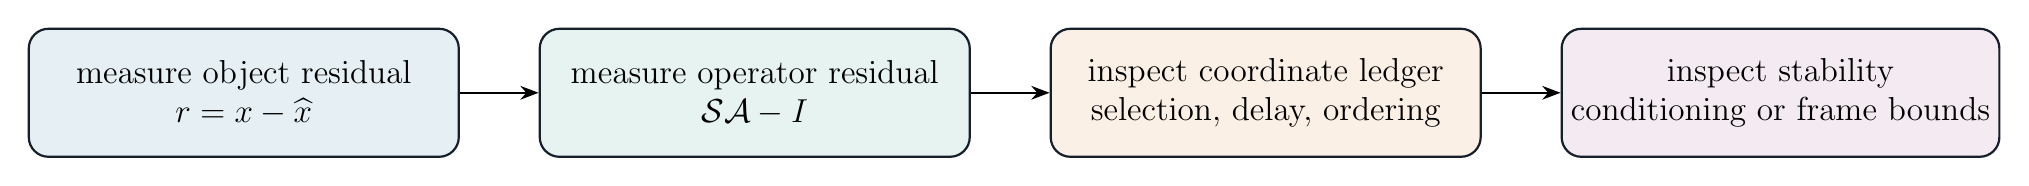
\begin{tikzpicture}[>=Stealth,node distance=7mm and 10mm,
 box/.style={rounded corners=2.5mm,draw=Ink,thick,minimum width=2.15in,minimum height=.64in,align=center,font=\large}]
\node[box,fill=PaleBlue] (r) {measure object residual\\$r=x-\widehat x$};
\node[box,fill=PaleTeal,right=of r] (op) {measure operator residual\\$\mathcal S\mathcal A-I$};
\node[box,fill=PaleOrange,right=of op] (coord) {inspect coordinate ledger\\selection, delay, ordering};
\node[box,fill=PaleMagenta,right=of coord] (cond) {inspect stability\\conditioning or frame bounds};
\draw[->,thick] (r)--(op); \draw[->,thick] (op)--(coord); \draw[->,thick] (coord)--(cond);
\end{tikzpicture}
\end{center}
\vfill
\Callout[PaleOrange]{A reconstruction residual is evidence, not merely a score. Its packet, spectral, spatial, or graph localization often reveals which part of the declared analysis--selection--synthesis chain is responsible.}

% Glossary II
\clearpage
\PageTitle[GLOSSARY II]{Vocabulary introduced by the expanded atlas}
\begin{multicols}{2}
\textbf{Oblique projector.} An idempotent projector that need not be self-adjoint; exact synthesis may hold without orthogonal energy partition.\par
\textbf{Condition number.} A sensitivity measure for an invertible coordinate map; large values signal amplification of coordinate perturbations.\par
\textbf{Commutator.} $[P,Q]=PQ-QP$, used here to test whether two packet families are compatible with a simple joint refinement.\par
\textbf{Tensor-product packet.} A multidimensional packet formed from coordinate packets along separate axes.\par
\textbf{Graph Fourier mode.} An eigenvector of a graph operator, usually a Laplacian, used as a spectral coordinate on a non-Euclidean domain.\par
\textbf{Mode atlas.} A coordinate family built from singular vectors, covariance eigenvectors, or another data-adapted modal decomposition.\par
\textbf{Tight frame.} A redundant family with a particularly simple exact synthesis law and controlled energy relation.\par
\textbf{Dual frame.} A synthesis family that reconstructs objects from redundant analysis coefficients.\par
\columnbreak
\textbf{Alias cancellation.} The synthesis-side cancellation of spectral replicas introduced by downsampling in a perfect-reconstruction bank.\par
\textbf{Best basis.} A complete pruned packet tree chosen by an additive cost; leaves may occur at different depths while exact synthesis remains possible.\par
\textbf{Rate--distortion curve.} Approximation error as a function of a retained-coordinate budget.\par
\textbf{Operator sparsity.} The extent to which transfer blocks vanish or concentrate in a chosen atlas.\par
\textbf{Quadratic interaction packet.} A contribution indexed by a pair of input packets and, after output projection, an output packet.\par
\textbf{Interaction hypergraph.} A visual representation of multi-input packet couplings that cannot be encoded by an ordinary transfer matrix alone.\par
\textbf{Object residual.} $x-\widehat x$, showing what the synthesized object omitted.\par
\textbf{Operator residual.} $\mathcal S\mathcal A-I$, showing whether the declared synthesis inverts the analysis before any particular input is chosen.\par
\end{multicols}
\vfill
\Callout[PaleTeal]{The expanded terminology is still organized by the same three questions: what coordinates were declared, what information was selected, and what synthesis law was used to return to the object space?}

% 44
\clearpage
\PageTitle[GLOSSARY]{A compact visual vocabulary}
\begin{multicols}{2}
\textbf{Packet.} A component $P_\alpha x$ selected by a projector.\par
\textbf{Complete packet system.} Pairwise annihilating projectors whose sum is the identity.\par
\textbf{Analysis.} The map $x\mapsto(P_\alpha x)_\alpha$ or an equivalent transformed coordinate tuple.\par
\textbf{Synthesis.} The inverse map that recombines all coordinates.\par
\textbf{Transfer block.} $P_\beta TP_\alpha$, the part of $T$ connecting two packets.\par
\textbf{Refinement.} Replacing a parent packet by a complete family of child packets.\par
\textbf{Polyphase channel.} One residue class of sample addresses after extraction and decimation.\par
\textbf{Perfect reconstruction.} An analysis--synthesis pair whose composition is identity, possibly with a declared delay.\par
\columnbreak
\textbf{Transform atlas.} Coordinates obtained from an invertible transform $U$.\par
\textbf{Coordinate selector.} A projector $E_\alpha$ that keeps specified transformed coordinates.\par
\textbf{Pulled-back projector.} $U^{-1}E_\alpha U$, acting in the original object space.\par
\textbf{Fourier packet.} A pulled-back selector of one bin or a disjoint frequency band.\par
\textbf{Wavelet packet.} A pulled-back selector of a scale--location or packet coefficient set.\par
\textbf{Exact reconstruction.} Every coordinate required by the declared complete atlas is retained.\par
\textbf{Approximation.} A selector, threshold, or model discards part of the complete coordinate tuple.\par
\textbf{Residual.} $r=x-\widehat x$, the object-level certificate of what reconstruction omitted.\par
\end{multicols}
\vfill
\Callout[PaleTeal]{The same vocabulary extends beyond finite signals whenever domains, convergence, topology, and operator closure are specified carefully. This guide restricts its numerical certificates to finite-dimensional examples and finite graphs.}

% 45
\clearpage
\PageTitle[READING MAP]{Where the formal proofs live in the technical series}
\begin{tabularx}{\linewidth}{>{\bfseries}p{2.2in} X X}
\toprule
Upstream work & Main material used here & Role in this guide \\
\midrule
Paper I: Foundations & packet systems, analysis/synthesis, transfer blocks, coordinate transport & universal grammar for decomposition and operator reconstruction \\
Paper II: Refinement and Compression & parent--child projectors, coordinate refinement maps, finite Fourier selector formulas & exact refinement and spectral-coordinate bridge \\
Paper V: Polyphase, Harmonic, and Group Structure & residue channels, polyphase matrices, perfect reconstruction, Haar banks, lifting, wavelet packets & multirate and wavelet realizations \\
Papers III--IV and VI--VIII & infinite completion, nonlinear transfer, geometry, harmonic structure, probability, and quantum extensions & context for graph, modal, frame, and nonlinear visualizations without replacing their formal hypotheses \\
Companion B: Reference Manual and Computational Atlas & notation, statement locations, source coordinates, test registry & lookup and audit layer for the full series \\
\bottomrule
\end{tabularx}
\vspace{0.24in}
\TwoBox{PaleBlue}{\textbf{What this visual guide does.}\par It gives a dependency-ordered picture of the shared mechanism and supplies finite numerical demonstrations.}{PaleOrange}{\textbf{What it does not do.}\par It does not replace the hypotheses, proofs, domain conditions, or status boundaries in the technical papers.}
\vfill
\Callout{A reader can use this guide first, then follow the topic-specific path into the formal series instead of reading the entire corpus linearly.}

% 46
\clearpage
\PageTitle[REPRODUCIBILITY]{How the visual atlas was generated and checked}
\begin{minipage}[t]{0.56\linewidth}
\textbf{Generated assets}
\begin{itemize}
\item 149 figures, each exported as vector PDF and high-resolution PNG;
\item deterministic one-dimensional signals, two-dimensional images, graph signals, matrices, and finite frame examples;
\item exact residue, Fourier, Haar, Daubechies, CDF 5/3, graph, frame, SVD/PCA, operator-block, phase--frequency, and nonlinear packet checks;
\item a CSV coordinate-atlas table and separate core, expanded, advanced, cross-domain, and combined JSON numerical-certificate ledgers;
\item Python source for every figure and identity test.
\end{itemize}
\textbf{Interpretation rule}
\begin{itemize}
\item algebraic residual $0$ means the finite computation is exactly zero;
\item residuals around $10^{-14}$ are consistent with double-precision roundoff;
\item nonzero edge and sparse-reconstruction errors are approximation metrics and are never used as perfect-reconstruction certificates.
\end{itemize}
\end{minipage}\hfill
\begin{minipage}[t]{0.40\linewidth}
\colorbox{PaleTeal}{\parbox{0.92\linewidth}{
\vspace{8pt}
\textbf{Representative residuals}
\begin{align*}
\text{packet synthesis} &=0,\\
\text{polyphase synthesis} &=0,\\
\text{operator block sum} &=0,\\
\text{Haar synthesis} &\approx4.44\times10^{-16},\\
\text{Fourier synthesis} &\approx1.08\times10^{-14},\\
\text{wavelet-packet synthesis} &\approx1.11\times10^{-15},\\
\text{2D Haar synthesis} &\approx6.66\times10^{-16},\\
\text{graph packet synthesis} &\approx7.77\times10^{-16},\\
\text{DB2 multilevel synthesis} &\approx2.00\times10^{-15},\\
\text{CDF 5/3 integer synthesis} &=0.
\end{align*}
\vspace{4pt}}}
\end{minipage}
\vfill
\Callout[PaleMagenta]{The release includes tests that regenerate the figures, verify the projector identities, and confirm that every figure named by the manuscript is present.}

% 47
\clearpage
\PageTitle[CLOSING VIEW]{The object is primary; the atlas is chosen for the question}
\begin{center}
\includegraphics[width=10.8in,height=4.25in,keepaspectratio]{32_unified_atlas.pdf}
\end{center}
\vspace{0.08in}
\begin{center}
\Large
\textbf{Decompose completely. Transfer through declared blocks. Refine without loss. Approximate only by an explicit selector. Reconstruct with a certificate.}
\end{center}
\vfill
\Callout{Fourier coordinates, wavelet coordinates, polyphase channels, and other invertible realizations are all available within this framework because each supplies a complete coordinate atlas and a corresponding family of pulled-back projectors.}

\end{document}
